%definira klasu dokumenta 
\documentclass[12pt]{report} 

%prostor izmedu naredbi \documentclass i \begin{document} se zove uvod. U njemu se nalaze naredbe koje se odnose na cijeli dokument

%osnovni LaTex ne može riješiti sve probleme, pa se koriste različiti paketi koji olakšavaju izradu željenog dokumenta
\usepackage[croatian]{babel} 
\usepackage{amssymb}
\usepackage{amsmath}
\usepackage{txfonts}
\usepackage{mathdots}
\usepackage{titlesec}
\usepackage{array}
\usepackage{lastpage}
\usepackage{etoolbox}
\usepackage{tabularray}
\usepackage{color, colortbl}
\usepackage{adjustbox}
\usepackage{geometry}
\usepackage[classicReIm]{kpfonts}
\usepackage{hyperref}
\usepackage{fancyhdr}

\usepackage{float}
\usepackage{setspace}
\restylefloat{table}


\patchcmd{\chapter}{\thispagestyle{plain}}{\thispagestyle{fancy}}{}{} %redefiniranje stila stranice u paketu fancyhdr

%oblik naslova poglavlja
\titleformat{\chapter}{\normalfont\huge\bfseries}{\thechapter.}{20pt}{\Huge}
\titlespacing{\chapter}{0pt}{0pt}{40pt}


\linespread{1.3} %razmak između redaka

\geometry{a4paper, left=1in, top=1in,}  %oblik stranice

\hypersetup{ colorlinks, citecolor=black, filecolor=black, linkcolor=black,	urlcolor=black }   %izgled poveznice


%prored smanjen između redaka u nabrajanjima i popisima
\newenvironment{packed_enum}{
	\begin{enumerate}
		\setlength{\itemsep}{0pt}
		\setlength{\parskip}{0pt}
		\setlength{\parsep}{0pt}
	}{\end{enumerate}}

\newenvironment{packed_item}{
	\begin{itemize}
		\setlength{\itemsep}{0pt}
		\setlength{\parskip}{0pt}
		\setlength{\parsep}{0pt}
	}{\end{itemize}}




%boja za privatni i udaljeni kljuc u tablicama
\definecolor{LightBlue}{rgb}{0.9,0.9,1}
\definecolor{LightGreen}{rgb}{0.9,1,0.9}

%Promjena teksta za dugačke tablice
\DefTblrTemplate{contfoot-text}{normal}{Nastavljeno na idućoj stranici}
\SetTblrTemplate{contfoot-text}{normal}
\DefTblrTemplate{conthead-text}{normal}{(Nastavljeno)}
\SetTblrTemplate{conthead-text}{normal}
\DefTblrTemplate{middlehead,lasthead}{normal}{Nastavljeno od prethodne stranice}
\SetTblrTemplate{middlehead,lasthead}{normal}

%podesavanje zaglavlja i podnožja

\pagestyle{fancy}
\lhead{Programsko inženjerstvo}
\rhead{$<$CodeShark$>$}
\lfoot{$<$DomeFanClub$>$}
\cfoot{stranica \thepage/\pageref{LastPage}}
\rfoot{\today}
\renewcommand{\headrulewidth}{0.2pt}
\renewcommand{\footrulewidth}{0.2pt}


\begin{document} 
	
	
	
	\begin{titlepage}
		\begin{center}
			\vspace*{\stretch{1.0}} %u kombinaciji s ostalim \vspace naredbama definira razmak između redaka teksta
			\LARGE Programsko inženjerstvo\\
			\large Ak. god. 2021./2022.\\
			
			\vspace*{\stretch{3.0}}
			
			\huge CodeShark\\
			\Large Dokumentacija, Rev. 2. 0\\
			
			\vspace*{\stretch{12.0}}
			\normalsize
			Grupa: DomeFanClub\\
			Voditelj: Marko Damjanić\\
			
			
			\vspace*{\stretch{1.0}}
			Datum predaje: 26. 10. 2021.\\
	
			\vspace*{\stretch{4.0}}
			
			Nastavnik: Hrvoje Nuić\\
		
		\end{center}

	
	\end{titlepage}

	
	\tableofcontents


	\chapter{Dnevnik promjena dokumentacije}
		
		
				
		
		\begin{longtblr}[
				label=none
			]{
				width = \textwidth, 
				colspec={|X[2]|X[13]|X[3]|X[3]|}, 
				rowhead = 1
			}
			\hline
			\textbf{Rev.}	& \textbf{Opis promjene/dodatka} & \textbf{Autori} & \textbf{Datum}\\[3pt] \hline
			0.1 & Napravljen predložak.	& Marko Damjanić & 26.10.2021. 		\\[3pt] \hline
			0.2 & Napravljen opis projekta	& Marko Damjanić & 7.11.2021. 		\\[3pt] \hline
			0.3 & Dodano u 3.1 : dionici i aktori & Fran Jelavić & 16.11.2021. 		\\[3pt] \hline
			0.4 & Dodano u 4 : uvod & Fran Jelavić & 16.11.2021. 		\\[3pt] \hline
			0.5 & Dodano u 3.11 : opis obrazaca uporabe & Luka Maros & 16.11.2021. 		\\[3pt] \hline
			0.6 & Dodano u 3.11 : opis obrazaca uporabe & Antonio Griparić & 16.11.2021. 		\\[3pt] \hline
			0.7 & Uspostavljena Baza podataka & Marko Damjanić & 16.11.2021. 		\\[3pt] \hline
			
			&  &  & \\[3pt] \hline	
		\end{longtblr}
	
	
	
	\chapter{Opis projektnog zadatka}
		
		\textbf{\textit{dio 1. revizije}}\\
		
		\textit{Na osnovi projektnog zadatka detaljno opisati korisničke zahtjeve. Što jasnije opisati cilj projektnog zadatka, razraditi problematiku zadatka, dodati nove aspekte problema i potencijalnih rješenja. Očekuje se minimalno 3, a poželjno 4-5 stranica opisa.	Teme koje treba dodatno razraditi u ovom poglavlju su:}
		\begin{packed_item}
			\item \textit{potencijalna korist ovog projekta}
			\item \textit{postojeća slična rješenja (istražiti i ukratko opisati razlike u odnosu na zadani zadatak). Dodajte slike koja predočavaju slična rješenja.}
			\item \textit{skup korisnika koji bi mogao biti zainteresiran za ostvareno rješenje.}
			\item \textit{mogućnost prilagodbe rješenja }
			\item \textit{opseg projektnog zadatka}
			\item \textit{moguće nadogradnje projektnog zadatka}
		\end{packed_item}
		
		\textit{Za pomoć pogledati reference navedene u poglavlju „Popis literature“, a po potrebi konzultirati sadržaj na internetu koji nudi dobre smjernice u tom pogledu.}
		\eject
		
		\section{Primjeri u \LaTeX u}
		
		\textit{Ovo potpoglavlje izbrisati.}\\

		U nastavku se nalaze različiti primjeri kako koristiti osnovne funkcionalnosti \LaTeX a koje su potrebne za izradu dokumentacije. Za dodatnu pomoć obratiti se asistentu na projektu ili potražiti upute na sljedećim web sjedištima:
		\begin{itemize}
			\item Upute za izradu diplomskog rada u \LaTeX u - \url{https://www.fer.unizg.hr/_download/repository/LaTeX-upute.pdf}
			\item \LaTeX\ projekt - \url{https://www.latex-project.org/help/}
			\item StackExchange za Tex - \url{https://tex.stackexchange.com/}\\
		
		\end{itemize} 	


		
		\noindent \underbar{podcrtani tekst}, \textbf{podebljani tekst}, 	\textit{nagnuti tekst}\\
		\noindent \normalsize primjer \large primjer \Large primjer \LARGE {primjer} \huge {primjer} \Huge primjer \normalsize
				
		\begin{packed_item}
			
			\item  primjer
			\item  primjer
			\item  primjer
			\item[] \begin{packed_enum}
				\item primjer
				\item[] \begin{packed_enum}
					\item[1.a] primjer
					\item[b] primjer
				\end{packed_enum}
				\item primjer
			\end{packed_enum}
			
		\end{packed_item}
		
		\noindent primjer url-a: \url{https://www.fer.unizg.hr/predmet/proinz/projekt}
		
		\noindent posebni znakovi: \# \$ \% \& \{ \} \_ 
		$|$ $<$ $>$ 
		\^{} 
		\~{} 
		$\backslash$ 
		
		
		\begin{longtblr}[
			label=none,
			entry=none
			]{
				width = \textwidth,
				colspec={|X[8,l]|X[8, l]|X[16, l]|}, 
				rowhead = 1,
			} %definicija širine tablice, širine stupaca, poravnanje i broja redaka naslova tablice
			\hline \multicolumn{3}{|c|}{\textbf{naslov unutar tablice}}	 \\ \hline[3pt]
			\SetCell{LightGreen}IDKorisnik & INT	&  	Lorem ipsum dolor sit amet, consectetur adipiscing elit, sed do eiusmod  	\\ \hline
			korisnickoIme	& VARCHAR &   	\\ \hline 
			email & VARCHAR &   \\ \hline 
			ime & VARCHAR	&  		\\ \hline 
			\SetCell{LightBlue} primjer	& VARCHAR &   	\\ \hline 
		\end{longtblr}
		

		\begin{longtblr}[
				caption = {Naslov s referencom izvan tablice},
				entry = {Short Caption},
			]{
				width = \textwidth, 
				colspec = {|X[8,l]|X[8,l]|X[16,l]|}, 
				rowhead = 1,
			}
			\hline
			\SetCell{LightGreen}IDKorisnik & INT	&  	Lorem ipsum dolor sit amet, consectetur adipiscing elit, sed do eiusmod  	\\ \hline
			korisnickoIme	& VARCHAR &   	\\ \hline 
			email & VARCHAR &   \\ \hline 
			ime & VARCHAR	&  		\\ \hline 
			\SetCell{LightBlue} primjer	& VARCHAR &   	\\ \hline 
		\end{longtblr}
	


		
		
		%unos slike
		\begin{figure}[H]
			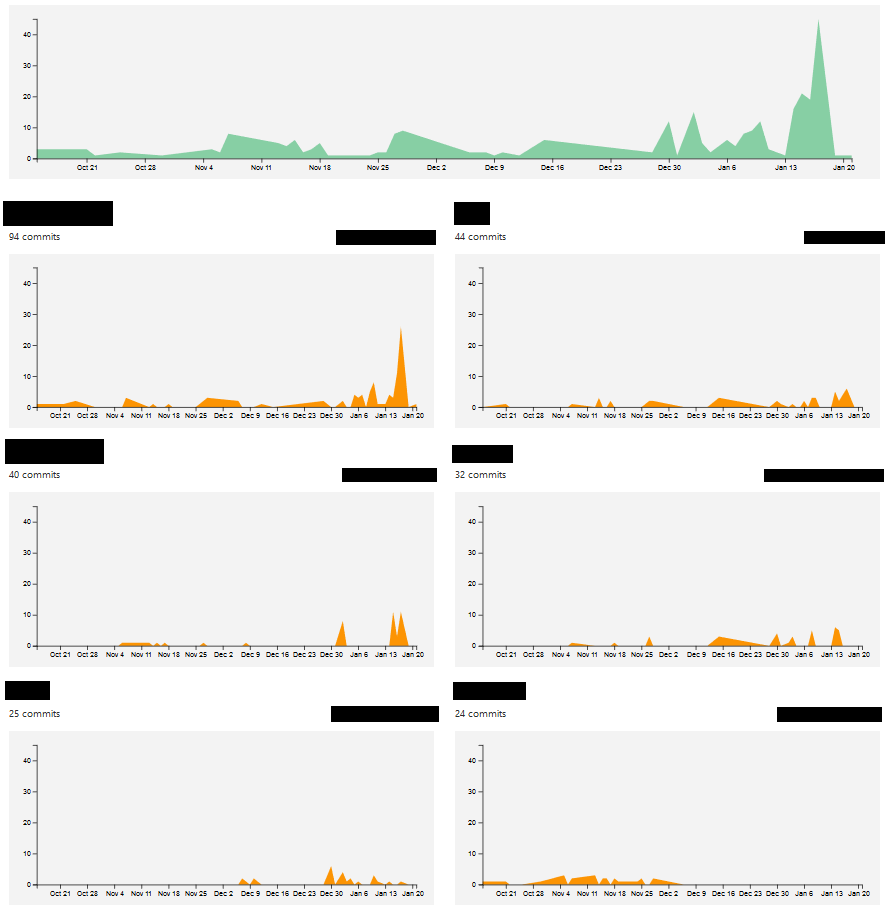
\includegraphics[scale=0.4]{slike/aktivnost.PNG} %veličina slike u odnosu na originalnu datoteku i pozicija slike
			\centering
			\caption{Primjer slike s potpisom}
			\label{fig:promjene}
		\end{figure}
		
		\begin{figure}[H]
			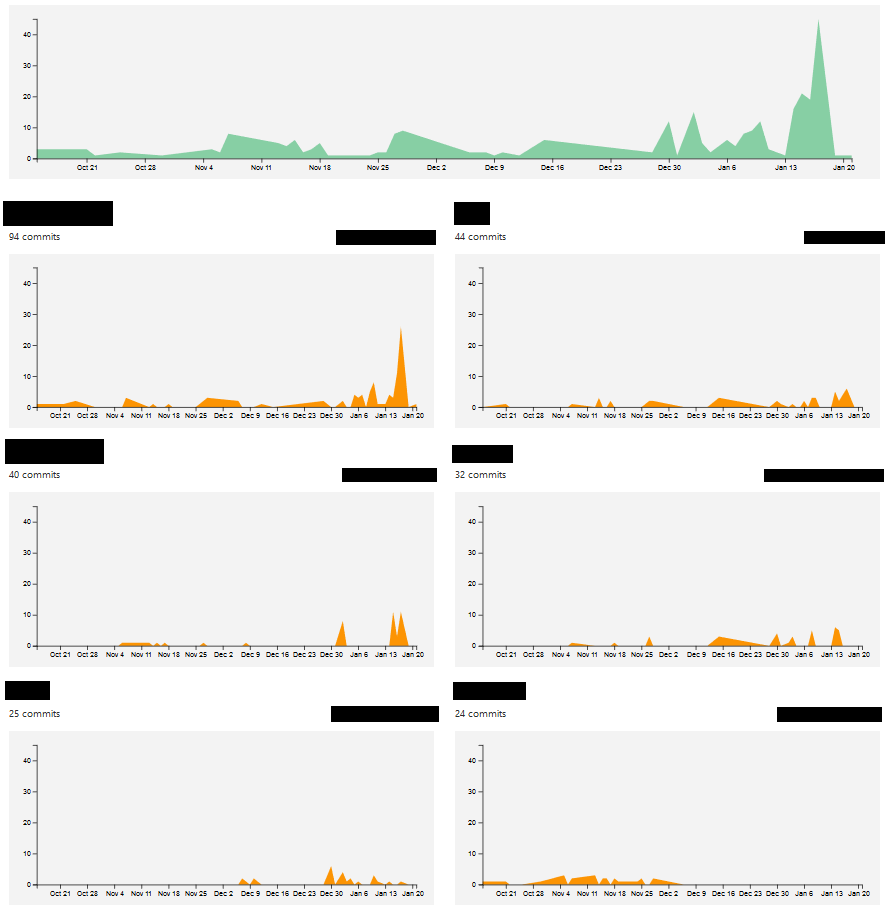
\includegraphics[width=\textwidth]{slike/aktivnost.PNG} %veličina u odnosu na širinu linije
			\caption{Primjer slike s potpisom 2}
			\label{fig:promjene2} %label mora biti drugaciji za svaku sliku
		\end{figure}
		
		Referenciranje slike \ref{fig:promjene2} u tekstu.
		
		\eject
		
	
	\chapter{Specifikacija programske potpore}
		
	\section{Funkcionalni zahtjevi}
			
			\noindent \textbf{Dionici:}
			
			\begin{packed_enum}
				
				\item Natjecatelj
				\item Voditelj
				\item Administrator				
				\item Razvojni tim
				
			\end{packed_enum}
			
			\noindent \textbf{Aktori i njihovi funkcionalni zahtjevi:}
			
			
			\begin{packed_enum}
				\item  \underbar{Neregistrirani/neprijavljeni korisnik (inicijator) može:}
				
				\begin{packed_enum}
					
					\item pretraživati natjecanja i pristupiti popisu zadataka s natjecanja i sudionika natjecanja
					\item pretraživati i čitati zadatke s natjecanja
					\item pristupiti informacijama tuđeg korisničkog profila:
					
					\begin{packed_enum}
						
					\item  korisničko ime, ime i prezime, i osvojene nagrade
					\item  statistike u što se ubraja broj točno riješenih i broj isprobanih zadataka
					\item  popis natjecanja na kojima je korisnik prisustvovao ili natjecanja koja je održavao
					
				
					\end{packed_enum}
					\item se registrirati u sustav, stvoriti novi korisnički račun za koji:
					
					\begin{packed_enum}
						
						\item  su mu potrebni korisničko ime, lozinka, ime i prezime te e-mail adresa
						\item  mora izabrati razinu pristupa "natjecatelj" ili "voditelj"
						
					\end{packed_enum}
				\end{packed_enum}
			
				\item  \underbar{Natjecatelj (inicijator) može:}
				
				\begin{packed_enum}
					
					\item pregledavati i mijenjati osobne podatke
					\item izbrisati svoj korisnički račun
					\item pristupiti zadatcima za vježbu i rješavati ih
					\item prijaviti i odjaviti se na natjecanja i pristupiti natjecanjima
					\item osvojiti nagrade
					\item pokrenuti virtualno natjecanje
					
				\end{packed_enum}
			
				\item  \underbar{Voditelj (inicijator) može:}
				
				\begin{packed_enum}
					
					\item pokrenuti i voditi vlastito natjecanje 
					
				\end{packed_enum}
				
				\item  \underbar{Administrator (inicijator) može:}
				
				\begin{packed_enum}
					
					\item vidjeti popis svih registriranih korisnika i njihovih osobnih podataka
					\item korisnike brisati i mijenjati im razinu pristupa aplikaciji (natjecatelj, voditelj)
					\item pristupiti statistici
					\item stvarati i brisati zadatke
					\item odobravati zahtjeve za razinu pristupa voditelja
					
				\end{packed_enum}
			
					
			\end{packed_enum}
			
			\eject 
			
			
				
			\subsection{Obrasci uporabe}
				
				\subsubsection{Opis obrazaca uporabe}

				\noindent \underbar{\textbf{UC1 - Registracija}}
					\begin{packed_item}
	
						\item \textbf{Glavni sudionik: } Korisnik
						\item  \textbf{Cilj:} Registracija u sustav
						\item  \textbf{Sudionici:} Baza podataka
						\item  \textbf{Preduvjet:} -
						\item  \textbf{Opis osnovnog tijeka:}
						
						\item[] \begin{packed_enum}
	
							\item Korisnik odabire opciju za registraciju
							\item Korisnik unosi potrebne korisnicke podatke
							\item Korisnik prima obavijest o uspjesnoj registraciji
						\end{packed_enum}
						
						\item  \textbf{Opis mogućih odstupanja:}
						
						\item[] \begin{packed_item}
	
							\item[2.a] Odabir vec zauzetog korisničkog imena i/ili e-maila, unos korisničkog
							podatka u nedozvoljenom formatu ili pruzanje neispravnoga e-maila
							\item[] \begin{packed_enum}
								
								\item Sustav obavještava korisnika o neuspjelom upisu i vraća ga na stra- 
								nicu za registraciju
								\item Korisnik mijenja potrebne podatke te završava unos ili odustaje od 
								registracije
								
							\end{packed_enum}
							
						\end{packed_item}
					\end{packed_item}

					\noindent \underbar{\textbf{UC2 - Prijava}}
					\begin{packed_item}
	
						\item \textbf{Glavni sudionik: } Korisnik
						\item  \textbf{Cilj:} Dobiti pristup korisničkom sučelju
						\item  \textbf{Sudionici:} Baza podataka
						\item  \textbf{Preduvjet:} Registracija
						\item  \textbf{Opis osnovnog tijeka:}
						
						\item[] \begin{packed_enum}
	
							\item Unos korisničkog imena i lozinke
							\item Potvrda o ispravnosti unesenih podataka
							\item Pristup korisničkim funkcijama
						\end{packed_enum}
						
						\item  \textbf{Opis mogućih odstupanja:}
						
						\item[] \begin{packed_item}
	
							\item[2.a] Neispravno korisničko ime/lozinka
							\item[] \begin{packed_enum}
								
								\item Sustav obavještava korisnika o neuspjelom upisu i vraća ga na stra- 
								nicu za registraciju
								
								
							\end{packed_enum}
							
						\end{packed_item}
					\end{packed_item}
					
					\noindent \underbar{\textbf{UC3 - Pregled mojeg profila}}
					\begin{packed_item}
	
						\item \textbf{Glavni sudionik: } Korisnik
						\item  \textbf{Cilj:} Pregledati osobne podatke
						\item  \textbf{Sudionici:} Baza podataka
						\item  \textbf{Preduvjet:} Korisnik je prijavljen
						\item  \textbf{Opis osnovnog tijeka:}
						
						\item[] \begin{packed_enum}
	
							\item Korisnik odabire opciju "Moj Profil"
							\item Aplikacija prikazuje osobne podatke korisnika
						\end{packed_enum}
						
						
					\end{packed_item}

					\noindent \underbar{\textbf{UC4 - Promjena podataka na mojem profilu}}
					\begin{packed_item}
	
						\item \textbf{Glavni sudionik: } Korisnik
						\item  \textbf{Cilj:} Promjeniti osobne podatke
						\item  \textbf{Sudionici:} Baza podataka
						\item  \textbf{Preduvjet:} Korisnik je prijavljen
						\item  \textbf{Opis osnovnog tijeka:}
						
						\item[] \begin{packed_enum}
	
							\item Korisnik odabire opciju "Uredi profil"
							\item Korisnik mijenja svoje osobne podatke
							\item Korisnik sprema promjene
							\item Baza podataka se ažurira
						\end{packed_enum}
						\item  \textbf{Opis mogućih odstupanja:}
						
						\item[] \begin{packed_item}
	
							\item[2.a] Korisnik promjeni svoje osobne podatke, ali ne odabire opciju "Spremi" 
							\item[] \begin{packed_enum}
								
								\item Sustav obavještava korisnika da nije spremio podatke prije izlaza iz prozora.
								
								
							\end{packed_enum}
							
						\end{packed_item}
						
						
					\end{packed_item}

					\noindent \underbar{\textbf{UC5 - Odjava iz sustava}}
					\begin{packed_item}
	
						\item \textbf{Glavni sudionik: } Korisnik
						\item  \textbf{Cilj:} Odjava iz sustava
						\item  \textbf{Sudionici:} Korisnik
						\item  \textbf{Preduvjet:} Korisnik je prijavljen
						\item  \textbf{Opis osnovnog tijeka:}
						
						\item[] \begin{packed_enum}
	
							\item Korisnik odabire opciju "Odjava"
							\item Sustav vraća korisnika na početnu stranicu
						\end{packed_enum}
						
						
					\end{packed_item}

					\noindent \underbar{\textbf{UC6 - Brisanje mojeg profila}}
					\begin{packed_item}
	
						\item \textbf{Glavni sudionik: } Korisnik
						\item  \textbf{Cilj:} Brisanje korisničkog profila
						\item  \textbf{Sudionici:} Baza podataka
						\item  \textbf{Preduvjet:} Korisnik je prijavljen
						\item  \textbf{Opis osnovnog tijeka:}
						
						\item[] \begin{packed_enum}
	
							\item Korisnik odabire opciju "Izbriši Moj Profil"
							\item Sustav odjavljuje korisnika i vraća ga na početnu stranicu
							\item Baza Podataka se ažurira
						\end{packed_enum}
						
						
					\end{packed_item}

					\noindent \underbar{\textbf{UC7 - Pregled zadataka}}
					\begin{packed_item}
	
						\item \textbf{Glavni sudionik: } Korisnik
						\item  \textbf{Cilj:} Pregledati sve dostupne zadatke za vježbu
						\item  \textbf{Sudionici:} Baza podataka
						\item  \textbf{Preduvjet:} -
						\item  \textbf{Opis osnovnog tijeka:}
						
						\item[] \begin{packed_enum}
	
							\item Korisnik odabire opciju "Zadaci"
							\item Korisniku se prikažu svi dostupni zadaci za vježbu
						\end{packed_enum}
						
						
					\end{packed_item}

					\noindent \underbar{\textbf{UC8 - Rješavanje zadataka za vježbu}}
					\begin{packed_item}
	
						\item \textbf{Glavni sudionik: } Korisnik
						\item  \textbf{Cilj:} Pokretanje i rješavanje zadataka za vježbu
						\item  \textbf{Sudionici:} Baza podataka
						\item  \textbf{Preduvjet:} Korisnik je prijavljen
						\item  \textbf{Opis osnovnog tijeka:}
						
						\item[] \begin{packed_enum}
	
							\item Korisnik odabire jedan od zadataka za vježbu
							\item Sustav prebacuje korisnika na stranicu za rješavanje zadataka
						\end{packed_enum}
						
						
					\end{packed_item}

					\noindent \underbar{\textbf{UC9 - Dodavanje zadataka}}
					\begin{packed_item}
	
						\item \textbf{Glavni sudionik: } Voditelj
						\item  \textbf{Cilj:} Dodati novi zadatak u bazu zadataka za vježbu
						\item  \textbf{Sudionici:} Baza podataka
						\item  \textbf{Preduvjet:} Korisnik mora imati ovlasti "Voditelj"
						\item  \textbf{Opis osnovnog tijeka:}
						
						\item[] \begin{packed_enum}
	
							\item Voditelj odabire opciju "Dodaj novi zadatak"
							\item Voditelj upisuje tekst,težinu,rješenje i vremensko ograničenje za zadatak
							\item Voditelj odabire opciju "Završi"
							\item Baza podataka se ažurira
						\end{packed_enum}

						\item  \textbf{Opis mogućih odstupanja:}
						
						\item[] \begin{packed_item}
	
							\item[2.a] Voditelj unosi podatke u nedozvoljenom formatu
							\item[] \begin{packed_enum}
								
								\item Sustav obavještava voditelja o neuspjelom upisu podataka
								\item Voditelj popravlja unose
								
							\end{packed_enum}
						\end{packed_item}
						
						
					\end{packed_item}

					\noindent \underbar{\textbf{UC10 - Pregled sudionika koji su rješavali određeni zadatak}}
					\begin{packed_item}
	
						\item \textbf{Glavni sudionik: } Natjecatelj
						\item  \textbf{Cilj:} Pregledati sudionike koji su rješavali određeni zadatak
						\item  \textbf{Sudionici:} Baza podataka
						\item  \textbf{Preduvjet:} Korisnik je prijavljen
						\item  \textbf{Opis osnovnog tijeka:}
						
						\item[] \begin{packed_enum}
	
							\item Natjecatelj odabire jedan od zadataka
							\item Natjecatelju se otvara lista svih koji su ga rješavali
						\end{packed_enum}
						
						
					\end{packed_item}

					\noindent \underbar{\textbf{UC11 - Brisanje zadataka}}
					\begin{packed_item}
	
						\item \textbf{Glavni sudionik: } Voditelj
						\item  \textbf{Cilj:} Izbrisati zadatak iz baze zadataka za vježbu
						\item  \textbf{Sudionici:} Baza podataka
						\item  \textbf{Preduvjet:} Korisnik mora imati ovlasti "Voditelj"
						\item  \textbf{Opis osnovnog tijeka:}
						
						\item[] \begin{packed_enum}
	
							\item Voditelj odabire jedan od zadataka za vježbu
							\item Voditelj odabire opciju "Izbriši zadatak"
							\item Baza podataka se ažurira
						\end{packed_enum}
						
						
					\end{packed_item}

					\noindent \underbar{\textbf{UC12 - Uređivanje zadataka za vježbu}}
					\begin{packed_item}
	
						\item \textbf{Glavni sudionik: } Voditelj
						\item  \textbf{Cilj:} Urediti zadatak iz baze zadataka za vježbu
						\item  \textbf{Sudionici:} Baza podataka
						\item  \textbf{Preduvjet:} Korisnik mora imati ovlasti "Voditelj"
						\item  \textbf{Opis osnovnog tijeka:}
						
						\item[] \begin{packed_enum}
	
							\item Voditelj odabire jedan od zadataka za vježbu 
							\item Voditelj odabire opciju "Uredi zadatak"
							\item Voditelj upisuje tekst,težinu,rješenje i vremensko ograničenje za zadatak
							\item Voditelj odabire opciju "Završi"
							\item Baza podataka se ažurira
						\end{packed_enum}

						\item  \textbf{Opis mogućih odstupanja:}
						
						\item[] \begin{packed_item}
	
							\item[2.a] Voditelj unosi podatke u nedozvoljenom formatu
							\item[] \begin{packed_enum}
								
								\item Sustav obavještava voditelja o neuspjelom upisu podataka
								\item Voditelj popravlja unose
								
							\end{packed_enum}
						\end{packed_item}
						
						
					\end{packed_item}

					\noindent \underbar{\textbf{UC13 - Pregled natjecanja}}
					\begin{packed_item}
	
						\item \textbf{Glavni sudionik: } Natjecatelj
						\item  \textbf{Cilj:} Pregledati listu svih natjecanja
						\item  \textbf{Sudionici:} Baza podataka
						\item  \textbf{Preduvjet:} Korisnik je prijavljen
						\item  \textbf{Opis osnovnog tijeka:}
						
						\item[] \begin{packed_enum}
	
							\item Korisnik odabire opciju "Natjecanja"
							\item Sustav prenosi korisnika na stranicu s kalendarom i listom natjecanja
						\end{packed_enum}
						
						
					\end{packed_item}

					\noindent \underbar{\textbf{UC14 - Pokretanje virtualnog natjecanja}}
					\begin{packed_item}
	
						\item \textbf{Glavni sudionik: } Natjecatelj
						\item  \textbf{Cilj:} Vježba putem virtualnih natjecanja
						\item  \textbf{Sudionici:} Baza podataka
						\item  \textbf{Preduvjet:} Korisnik je prijavljen
						\item  \textbf{Opis osnovnog tijeka:}
						
						\item[] \begin{packed_enum}
	
							\item Voditelj odabire opciju "Natjecanja"
							\item Korisnik odabire "Novo virtualno natjecanje"
							\item Korisnik započinje rješavanje natjecanja
						\end{packed_enum}
						
						
					\end{packed_item}

					\noindent \underbar{\textbf{UC15 - Dodavanje natjecanja}}
					\begin{packed_item}
	
						\item \textbf{Glavni sudionik: }Voditelj
						\item  \textbf{Cilj:} Dodati natjecanje
						\item  \textbf{Sudionici:} Baza podataka
						\item  \textbf{Preduvjet:} Korisnik mora biti prijavljen i imati ulogu voditelja
						\item  \textbf{Opis osnovnog tijeka:}
						
						\item[] \begin{packed_enum}
	
							\item Voditelj odabire karticu "Natjecanja"
							\item Voditelj dodaje novo natjecanje
							\item Voditelj unosi potrebne podatke o natjecanju
							\item Promjene se upisuju u bazu podataka
						\end{packed_enum}
						
						\item  \textbf{Opis mogućih odstupanja:}
						
						\item[] \begin{packed_item}
	
							\item[3.a] Voditelj unosi podatke u nedozvoljenom formatu
							\item[] \begin{packed_enum}
								
								\item Sustav obavještava voditelja o neuspjelom upisu podataka
								\item Voditelj popravlja neispravne unose i stvara natjecanje ili odustaje od stvaranja natjecanja
								
							\end{packed_enum}
						\end{packed_item}
					\end{packed_item}
				
					\noindent \underbar{\textbf{UC16 - Pokretanje natjecanja}}
					\begin{packed_item}
						
						\item \textbf{Glavni sudionik: }Voditelj
						\item  \textbf{Cilj:} Pokrenuti natjecanje
						\item  \textbf{Sudionici:} Baza podataka
						\item  \textbf{Preduvjet:} Korisnik mora biti prijavljen i imati ulogu voditelja
						\item  \textbf{Opis osnovnog tijeka:}
						
						\item[] \begin{packed_enum}
							
							\item Voditelj odabire karticu "Natjecanja"
							\item Voditelj odabire jedno od svojih natjecanja
							\item Voditelj pokreće natjecanje
						\end{packed_enum}
					\end{packed_item}
				
					\noindent \underbar{\textbf{UC17 - Prijava na natjecanje}}
					\begin{packed_item}
						
						\item \textbf{Glavni sudionik: }Natjecatelj
						\item  \textbf{Cilj:} Prijaviti se na nadolazeće natjecanje
						\item  \textbf{Sudionici:} Baza podataka
						\item  \textbf{Preduvjet:} Korisnik mora biti prijavljen
						\item  \textbf{Opis osnovnog tijeka:}
						
						\item[] \begin{packed_enum}
							
							\item Natjecatelj odabire karticu "Natjecanja"
							\item Natjecatelj odabire jedno od nadolazećih natjecanja
							\item Natjecatelj se prijavljuje na odabrano natjecanje
						\end{packed_enum}
					\end{packed_item}
				
					\noindent \underbar{\textbf{UC18 - Pristupanje natjecanju}}
					\begin{packed_item}
						
						\item \textbf{Glavni sudionik: }Natjecatelj
						\item  \textbf{Cilj:} Pristupiti natjecanju
						\item  \textbf{Sudionici:} Baza podataka
						\item  \textbf{Preduvjet:} Korisnik mora biti prijavljen u sustav i na natjecanje koje je trenutno aktivno
						\item  \textbf{Opis osnovnog tijeka:}
						
						\item[] \begin{packed_enum}
							
							\item Natjecatelj odabire karticu "Natjecanja"
							\item Natjecatelj odabire jedno od trenutno aktivnih natjecanja na koje je prijavljen
							\item Natjecatelj pristupa natjecanju
						\end{packed_enum}
					\end{packed_item}
				
					\noindent \underbar{\textbf{UC19 - Odjava s natjecanja}}
					\begin{packed_item}
						
						\item \textbf{Glavni sudionik: }Natjecatelj
						\item  \textbf{Cilj:} Odjaviti se s natjecanja
						\item  \textbf{Sudionici:} Baza podataka
						\item  \textbf{Preduvjet:} Korisnik mora biti prijavljen u sustav i na natjecanje
						\item  \textbf{Opis osnovnog tijeka:}
						
						\item[] \begin{packed_enum}
							
							\item Natjecatelj odabire karticu "Natjecanja"
							\item Natjecatelj odabire jedno od nadolazećih natjecanja na koje je prijavljen
							\item Natjecatelj se odjavljuje s odabranog natjecanja
						\end{packed_enum}
					\end{packed_item}
				
					\noindent \underbar{\textbf{UC20 - Uređivanje natjecanja}}
					\begin{packed_item}
						
						\item \textbf{Glavni sudionik: }Voditelj
						\item  \textbf{Cilj:} Urediti natjecanje
						\item  \textbf{Sudionici:} Baza podataka
						\item  \textbf{Preduvjet:} Korisnik mora biti prijavljen i imati ulogu voditelja
						\item  \textbf{Opis osnovnog tijeka:}
						
						\item[] \begin{packed_enum}
							
							\item Voditelj odabire karticu "Natjecanja"
							\item Voditelj odabire jedno od svojih natjecanja
							\item Voditelj uređuje pojedinosti svog natjecanja
							\item Promjene se upisuju u bazu podataka
						\end{packed_enum}
						
						\item  \textbf{Opis mogućih odstupanja:}
						
						\item[] \begin{packed_item}
							
							\item[3.a] Voditelj unosi podatke u nedozvoljenom formatu
							\item[] \begin{packed_enum}
								
								\item Sustav obavještava voditelja o neuspjelom upisu podataka
								\item Voditelj popravlja neispravne unose i uspješno uređuje natjecanje ili odustaje od uređivanja natjecanja
								
							\end{packed_enum}
						\end{packed_item}
					\end{packed_item}
				
					\noindent \underbar{\textbf{UC21 - Pregled sudionika na natjecanju}}
					\begin{packed_item}
						
						\item \textbf{Glavni sudionik: }Korisnik
						\item  \textbf{Cilj:} Pregledati natjecatelje koji su sudjelovali na natjecanju
						\item  \textbf{Sudionici:} Baza podataka
						\item  \textbf{Preduvjet:} -
						\item  \textbf{Opis osnovnog tijeka:}
						
						\item[] \begin{packed_enum}
							
							\item Korisnik odabire karticu "Natjecanja"
							\item Korisnik odabire jedno od prošlih natjecanja
							\item Prikazuje se lista natjecatelja koji su sudjelovali na odabranom natjecanju
						\end{packed_enum}
					\end{packed_item}
				
					\noindent \underbar{\textbf{UC22 - Brisanje natjecanja}}
					\begin{packed_item}
						
						\item \textbf{Glavni sudionik: }Administrator
						\item  \textbf{Cilj:} Obrisati postojeće natjecanje
						\item  \textbf{Sudionici:} Baza podataka
						\item  \textbf{Preduvjet:} Korisnik mora biti prijavljen i imati ulogu administratora
						\item  \textbf{Opis osnovnog tijeka:}
						
						\item[] \begin{packed_enum}
							
							\item Administrator odabire karticu "Natjecanja"
							\item Administrator odabire jedno od natjecanja
							\item Administrator briše odabrano natjecanje
							\item Natjecanje se briše iz baze podataka
						\end{packed_enum}
					\end{packed_item}
				
					\noindent \underbar{\textbf{UC23 - Dohvat učitanog rješenja zadatka s natjecanja}}
					\begin{packed_item}
						
						\item \textbf{Glavni sudionik: }Natjecatelj
						\item  \textbf{Cilj:} Dohvatiti učitano rješenje zadatka nekog od natjecatelja koji je sudjelovao na natjecanju
						\item  \textbf{Sudionici:} Baza podataka
						\item  \textbf{Preduvjet:} Korisnik mora biti prijavljen i imati potpuno točno riješen konkretan zadatak
						\item  \textbf{Opis osnovnog tijeka:}
						
						\item[] \begin{packed_enum}
							
							\item Natjecatelj odabire karticu "Natjecanja"
							\item Natjecatelj odabire jedno od prošlih natjecanja
							\item Natjecatelj odabire jedan od zadataka s odabranog natjecanja
							\item Natjecatelj dohvaća rješenje zadatka
						\end{packed_enum}
					\end{packed_item}
				
					\noindent \underbar{\textbf{UC24 - Završetak natjecanja}}
					\begin{packed_item}
						
						\item \textbf{Glavni sudionik: }Natjecatelj
						\item  \textbf{Cilj:} Završiti s natjecanjem
						\item  \textbf{Sudionici:} Baza podataka
						\item  \textbf{Preduvjet:} Korisnik mora biti prijavljen i morao je pristupiti natjecanju
						\item  \textbf{Opis osnovnog tijeka:}
						
						\item[] \begin{packed_enum}
							
							\item Natjecatelj odabire karticu "Natjecanja"
							\item Natjecatelj odabire jedno od trenutno aktivnih natjecanja na koje je prijavljen
							\item Natjecatelj pristupa natjecanju
							\item Nakon rješavanja zadataka, a prije isteka vremena, natjecatelj završava natjecanje
						\end{packed_enum}
					\end{packed_item}
				
					\noindent \underbar{\textbf{UC25 - Pregled ostalih korisnika}}
					\begin{packed_item}
						
						\item \textbf{Glavni sudionik: }Korisnik
						\item  \textbf{Cilj:} Pregled profila ostalih korisnika
						\item  \textbf{Sudionici:} Baza podataka
						\item  \textbf{Preduvjet:} -
						\item  \textbf{Opis osnovnog tijeka:}
						
						\item[] \begin{packed_enum}
							
							\item Korisnik odabire karticu "Korisnici"
							\item Prikazuje se lista svih registriranih natjecatelja i voditelja
						\end{packed_enum}
					\end{packed_item}
				
					\noindent \underbar{\textbf{UC26 - Promjena ovlasti korisniku}}
					\begin{packed_item}
						
						\item \textbf{Glavni sudionik: }Administrator
						\item  \textbf{Cilj:} Promjeniti ovlasti korisniku
						\item  \textbf{Sudionici:} Baza podataka
						\item  \textbf{Preduvjet:} Korisnik mora biti prijavljen i imati ulogu administratora
						\item  \textbf{Opis osnovnog tijeka:}
						
						\item[] \begin{packed_enum}
							
							\item Administrator odabire karticu "Korisnici"
							\item Administrator odabire korisnika
							\item Administrator mijenja odabranom korisniku ovlasti
							\item Promjene se upisuju u bazu podataka
						\end{packed_enum}
					\end{packed_item}
				
					\noindent \underbar{\textbf{UC27 - Pregled statistike pojedinog korisnika}}
					\begin{packed_item}
						
						\item \textbf{Glavni sudionik: }Korisnik
						\item  \textbf{Cilj:} Pregledati statistiku pojedinog korisnika
						\item  \textbf{Sudionici:} Baza podataka
						\item  \textbf{Preduvjet:} -
						\item  \textbf{Opis osnovnog tijeka:}
						
						\item[] \begin{packed_enum}
							
							\item Korisnik odabire karticu "Korisnici"
							\item Korisnik odabire određenog korisnika s liste
							\item Prikazuje se statistika odabranog korisnika
						\end{packed_enum}
					\end{packed_item}
				
					\noindent \underbar{\textbf{UC28 - Pregled svih učitanih rješenja nekog natjecatelja}}
					\begin{packed_item}
						
						\item \textbf{Glavni sudionik: }Natjecatelj
						\item  \textbf{Cilj:} Pregledati sva učitana rješenja natjecatelja koji je sudjelovao na natjecanju
						\item  \textbf{Sudionici:} Baza podataka
						\item  \textbf{Preduvjet:} Korisnik mora biti prijavljen
						\item  \textbf{Opis osnovnog tijeka:}
						
						\item[] \begin{packed_enum}
							
							\item Natjecatelj odabire karticu "Natjecanja"
							\item Natjecatelj odabire jedno od prošlih natjecanja
							\item Natjecatelj odabire jednog od natjecatelja koji je sudjelovao na natjecanju
							\item Prikazuju se sva učitana rješenja odabranog natjecatelja
						\end{packed_enum}
					\end{packed_item}
				
					\noindent \underbar{\textbf{UC29 - Promjena osobnih podataka korisniku}}
					\begin{packed_item}
						
						\item \textbf{Glavni sudionik: }Administrator
						\item  \textbf{Cilj:} Promijniti osobne podatke korisniku
						\item  \textbf{Sudionici:} Baza podataka
						\item  \textbf{Preduvjet:} Korisnik mora biti prijavljen i imati ulogu administratora
						\item  \textbf{Opis osnovnog tijeka:}
						
						\item[] \begin{packed_enum}
							
							\item Administrator odabire karticu "Korisnici"
							\item Administrator odabire određenog korisnika
							\item Administrator mijenja željene osobne podatke korisniku
							\item Promjene se upisuju u bazu podataka
						\end{packed_enum}
						
						\item  \textbf{Opis mogućih odstupanja:}
						
						\item[] \begin{packed_item}
							
							\item[3.a] Voditelj unosi podatke u nedozvoljenom formatu
							\item[] \begin{packed_enum}
								
								\item Sustav obavještava administratora o neuspjelom upisu podataka
								\item Administrator popravlja neispravne unose i uspješno mijenja osobne podatke odabranog korisnika ili odustaje od promjena
								
							\end{packed_enum}
						\end{packed_item}
					\end{packed_item}
				
					\noindent \underbar{\textbf{UC30 - Potvrda promjene uloge voditelja}}
					\begin{packed_item}
						
						\item \textbf{Glavni sudionik: }Administrator
						\item  \textbf{Cilj:} Potvrditi promjenu uloge voditelju
						\item  \textbf{Sudionici:} Baza podataka
						\item  \textbf{Preduvjet:} Korisnik mora biti prijavljen i imati ulogu administratora
						\item  \textbf{Opis osnovnog tijeka:}
						
						\item[] \begin{packed_enum}
							
							\item Administrator odabire karticu "Korisnici"
							\item Administrator odabire određenog korisnika
							\item Administrator potvrđuje korisniku promjenu uloge u voditelja natjecanja
							\item Promjene se upisuju u bazu podataka
						\end{packed_enum}
					\end{packed_item}
					
				\subsubsection{Dijagrami obrazaca uporabe}
					
					\textit{Prikazati odnos aktora i obrazaca uporabe odgovarajućim UML dijagramom. Nije nužno nacrtati sve na jednom dijagramu. Modelirati po razinama apstrakcije i skupovima srodnih funkcionalnosti.}
				\eject		
				
			\subsection{Sekvencijski dijagrami}
				
				\textbf{\textit{dio 1. revizije}}\\
				
				\textit{Nacrtati sekvencijske dijagrame koji modeliraju najvažnije dijelove sustava (max. 4 dijagrama). Ukoliko postoji nedoumica oko odabira, razjasniti s asistentom. Uz svaki dijagram napisati detaljni opis dijagrama.}
				\eject
	
		\section{Ostali zahtjevi}
		
			\textbf{\textit{dio 1. revizije}}\\
		 
			 \textit{Nefunkcionalni zahtjevi i zahtjevi domene primjene dopunjuju funkcionalne zahtjeve. Oni opisuju \textbf{kako se sustav treba ponašati} i koja \textbf{ograničenja} treba poštivati (performanse, korisničko iskustvo, pouzdanost, standardi kvalitete, sigurnost...). Primjeri takvih zahtjeva u Vašem projektu mogu biti: podržani jezici korisničkog sučelja, vrijeme odziva, najveći mogući podržani broj korisnika, podržane web/mobilne platforme, razina zaštite (protokoli komunikacije, kriptiranje...)... Svaki takav zahtjev potrebno je navesti u jednoj ili dvije rečenice.}
			 
			 
			 
	
	\chapter{Arhitektura i dizajn sustava}
		
		\noindent Arhitekturu je moguće podijeliti na tri podsustava:
	\begin{itemize}
		\item 	Web poslužitelj
		\item 	Web aplikacija
		\item 	Baza podataka	
	\end{itemize}
		
		\underline{\textit{Web preglednik}} je program koji korisniku omogućuje pregled web-stranica i multimedijskog sadržaja vezanog uz njih. Korisnik putem web preglednika šalje zahtjev web poslužitelju te mu web preglednik kao interpreter prevodi web-stranicu i njezin sadržaj u format koji je korisniku razumljiv. \\
		\underline{\textit{Web poslužitelj}} temelj je rada web aplikacije te je njegov glavni zadatak omogućiti komunikaciju klijenta s aplikacijom. Komunikacija se ostvaruje preko protokola HTTP (engl. \textit{Hyper Text Transfer Protocol}), koji služi za prijenos informacija na webu. Web aplikacija se pokreće preko poslužitelja koji joj prosljeđuje zahtjev od strane korisnika. \\
		\underline{\textit{Web aplikacija}} služi za obradu korisničkih zahtjeva. Ovisno o zahtjevu, web aplikacija tijekom obrade zahtjeva pristupa bazi podataka te korisniku vraća odgovor u obliku HTML (engl. \textit{HyperText Markup Language}) dokumenta koji se prikazuje preko web preglednika. \\
		Codeshark web aplikacija bazirana je na programskom jeziku Python-u za razvoj \textit{backend}-a, zajedno s JavaScript-om uz biblioteku React za razvoj \textit{frontend}-a. Kao razvojno okruženje koristio se Microsoft Visual Studio. \\
		Arhitektura sustava temelji se na konceptu MVC-a (Model-View-Controller). Karakteristika MVC koncepta je nezavisan razvoj pojedinih dijelova aplikacije što za posljedicu ima jednostavnije ispitivanje kao i jednostavno razvijanje i dodavanje novih svojstava u sustav. \\
		
		\noindent MVC koncept sastoji se od:
		
		\begin{itemize}
			\item \textbf{Model} - Središnja komponenta sustava. Predstavlja dinamičke strukture podataka, neovisne o korisničkom sučelju. Izravno upravlja podacima, logikom i pravilima aplikacije. Ujedno i prima ulazne podatke od Controller-a.
			\item \textbf{View} - Bilo kakav prikaz podataka, poput grafa. Mogući su različiti prikazi iste informacije poput grafičkog ili tabličnog prikaza podataka.
			\item \textbf{Controller} - Prima ulaze i prilagođava ih za prosljeđivanje Model-u ili View-u. Upravlja korisničkim zahtjevima i temeljem njih izvodi daljnju interakciju s ostalim elementima sustava.
		\end{itemize}
		
				
		\section{Baza podataka}
		
		
		
		\noindent Za potrebe našeg sustava koristit  ćemo relacijsku bazu podataka koja svojom strukturom olakšava baratanju potrebnih podataka. Gradivna jedinka baze je relacija, odnosno tablica koja je definirana svojim imenom i skupom atributa. Zadaća baze podataka je brza i jednostavna pohrana, izmjena i dohvat podataka za daljnju obradu.
		Baza podataka ove aplikacije sastoji se od sljedećih entiteta:
		\begin{packed_item}
			\item Korisnik
			\item Natjecanje
			\item Zadatak
			\item Test-Primjeri
			\item Upload-Rjesenja
			\item Virtualno-Natjecanje
			\item Trofej
			\item Sudjeluje-Na
			\item Je-Osvojio
			\item Klasa-Natjecanja
		\end{packed_item}
		\subsection{Opis Tablica}
		\noindent \textbf{Korisnik} \space \space Ovaj entitet sadržava sve važne informacije o korisniku aplikacije.
		Sadrži atribute: Korisnikov ID, Korisničko ime, lozinku, ime, prezime, sliku profila, email, titulu i korisnikovu razinu ovlasti. Ovaj entitet u vezi je
		One-to-Many s entitetom Natjecanje preko ID-a korisnika (AutorID), u vezi One-to-Many s entitetom Zadatak preko ID-a korisnika (AutorID), u vezi Many-to-Many s  Je-Osvojio preko ID-a korisnika, u vezi Many-to-Many s  Sudjeluje-na preko ID-a korisnika, u vezi One-to-Many s entitetom Upload-Rjesenja preko ID-a korisnika  te u vezi One-to-Many s entitetom VirtNatjecanje preko ID-a korisnika.
		
		
		\begin{longtblr}[
			label=none,
			entry=none
			]{
				width = \textwidth,
				colspec={|X[6,l]|X[6, l]|X[20, l]|}, 
				rowhead = 1,
			} %definicija širine tablice, širine stupaca, poravnanje i broja redaka naslova tablice
			\hline \multicolumn{3}{|c|}{\textbf{Korisnik}}	 \\ \hline[3pt]
			\SetCell{LightGreen}Korisnik ID & INT	&  jedinstveni indikator korisnika  	\\ \hline
			KorisnickoIme	& VARCHAR & identificirajuće ime korisnika  	\\ \hline 
			Lozinka	& VARCHAR & hash lozinke 	\\ \hline
			SlikaProfila	& VARCHAR &  slika profila korisnika 	\\ \hline 
			Ime & VARCHAR	&  ime korisnika		\\ \hline 
			Prezime & VARCHAR	&  prezime korisnika		\\ \hline 
			Email & VARCHAR & email korisnika  \\ \hline 
			Titula	& VARCHAR & prilagođena titula korisnika  	\\ \hline  
			NivouPrava	& INT & razina ovlasti korisnika  	\\ \hline
			Token	& VARCHAR & token napravljen za korisnika 	\\ \hline  
			Token Generiran	& TIMESTAMP & vrijeme kada je token generiran\\ \hline  
			Aktivan	& Boolean & stanje verifikacije korisnika  	\\ \hline    
			
		\end{longtblr}
		
		\noindent \textbf{Natjecanje} \space \space Ovaj entitet sadržava sve važne informacije o održavanju natjecanja.
		Sadrži atribute:  ID Natjecanja, ime natjecanja, tekst natjecanja, vrijeme kraja natjecanja, vrijeme početka natjecanja, sliku trofeja, broj zadataka, ID autora natjecanja, ID klase natjecanja, ID trofeja. Ovaj entitet u vezi je	Many-to-One s entitetom Korisnik preko ID-a korisnika (AutorID), u vezi One-to-Many s entitetom Zadatak preko ID-a natjecanja , u vezi One-to-Many s  VirtNatjecanje preko ID-a natjecanja, u vezi One-to-One s  entitetom Trofej preko ID-a trofeja te u vezi Many-to-One s entitetom IDKlasaNatjecanja preko ID-a klase natjecanja.
		
		
		\begin{longtblr}[
			label=none,
			entry=none
			]{
				width = \textwidth,
				colspec={|X[6,l]|X[6, l]|X[20, l]|}, 
				rowhead = 1,
			} %definicija širine tablice, širine stupaca, poravnanje i broja redaka naslova tablice
			\hline \multicolumn{3}{|c|}{\textbf{Natjecanje}}	 \\ \hline[3pt]
			\SetCell{LightGreen}NatjecanjeID & INT	&  jedinstveni indikator natjecanja  	\\ \hline
			ImeNatjecanja	& VARCHAR & identificirajuće ime natjecanja  	\\ \hline 
			Tekst Natjecanja	& VARCHAR & sadržaj teksta natjecanja 	\\ \hline
			VrijemeKraj	& TIMESTAMP & vrijeme završetka natjecanja 	\\ \hline 
			VrijemePoc & TIMESTAMP	&  vrijeme početka natjecanje		\\ \hline 
			SlikaTrofeja & VARCHAR	&  sličica trofeja		\\ \hline 
			BrojZadataka & INT & broj zadataka u natjecanju  \\ \hline 
			\SetCell{LightBlue} AutorID	& INT & autorov Korisnik ID (korisnik.KorisnikID) 	\\ \hline  
			\SetCell{LightBlue} ID Klase Natjecanja & INT & ID Klase Natjecanja (klasanatjecanja.IDKlaseNatjecanja)  	\\ \hline  
			\SetCell{LightBlue} TrofejID	& INT & Trofej ID (trofej.TrofejID)   	\\ \hline 
		\end{longtblr}
		
		\noindent \textbf{Zadatak} \space \space Ovaj entitet sadržava sve važne informacije o zadacima.
		Sadrži atribute:  Zadatak ID, ime zadatka, tekst zadatka, bodovi zadatka, maksimalno vrijeme izvršavanja zadatka, privatnost zadatka, slag naziv zadatka, id autora , id natjecanja(opcionalno). Ovaj entitet u vezi je	Many-to-One s entitetom Korisnik preko ID-a korisnika (AutorID), u vezi Many-to-One s entitetom Natjecanje preko ID-a natjecanja , u vezi One-to-Many s  TestPrimjeri preko ID-a zadatka, u vezi One-to-Many s  entitetom UploadRjesenja preko ID-a zadatka te u 4 veze One-to-Many s entitetom VirtNatjecanje preko ID-a zadataka.
		
		\begin{longtblr}[
			label=none,
			entry=none
			]{
				width = \textwidth,
				colspec={|X[6,l]|X[6, l]|X[20, l]|}, 
				rowhead = 1,
			} %definicija širine tablice, širine stupaca, poravnanje i broja redaka naslova tablice
			\hline \multicolumn{3}{|c|}{\textbf{Zadatak}}	 \\ \hline[3pt]
			\SetCell{LightGreen}ZadatakID & INT	&  jedinstveni indikator zadatka  	\\ \hline
			ImeZadatka	& VARCHAR & identificirajući naziv zadatka  \\ \hline
			Bodovi	& INT & broj bodova(težina 1-5)	\\ \hline
			MaxVrijeme Izvrs	& NUMERIC &  maksimalno vrijeme izvršavanja programa 	\\ \hline 
			TekstZadatka & VARCHAR	&  sadržaj teksta zadatka		\\ \hline 
			Privatnost & Boolean	&  stanje privatnosti zadatka	\\ \hline 
			Slag & VARCHAR & slag verzija naziva zadatka  \\ \hline 
			\SetCell{LightBlue} AutorID	& INT & autorov Korisnik ID (korisnik.KorisnikID)  	\\ \hline  
			\SetCell{LightBlue} NatjecanjeID & INT &(opcionalno) Natjecanje ID (natjecanje.NatjecanjeID)  	\\ \hline  
			
		\end{longtblr}
		
		\noindent \textbf{Test Primjeri} \space \space Ovaj entitet sadržava sve važne informacije o testnim primjerima za zasebne zadatke.
		Sadrži atribute:  Zadatak ID, ulaz testa, izlaz testa. Ovaj entitet u vezi je	Many-to-One s entitetom Zadatak preko ID-a zadatka.
		
		\begin{longtblr}[
			label=none,
			entry=none
			]{
				width = \textwidth,
				colspec={|X[6,l]|X[6, l]|X[20, l]|}, 
				rowhead = 1,
			} %definicija širine tablice, širine stupaca, poravnanje i broja redaka naslova tablice
			\hline \multicolumn{3}{|c|}{\textbf{Test Primjeri}}	 \\ \hline[3pt]
			\SetCell{LightGreen}Ulaz & VARCHAR	&  ulaz testa  	\\ \hline
			\SetCell{LightGreen}Zadatak ID	& INT & Zadatak ID (zadatak.ZadatakID)  	\\ \hline 
			Izlaz	& VARCHAR & željeni izlaz testa	\\ \hline
			
		\end{longtblr}
		
		\noindent \textbf{Upload Rjesenja} \space \space Ovaj entitet sadržava sve informacije koje su bitne oko uploada rješenja na zadatak.
		Sadrži atribute:  Zadatak ID, korisnikov id, vrijeme predaje rješenja, predano rješenje, prolaznost, prosječno vrijeme izvršavanja, aktivnost natjecanja. Ovaj entitet u vezi je	Many-to-One s entitetom Korisnik preko ID-a korisnika  te u vezi Many-to-One s entitetom Zadatak preko ID-a zadatka.
		
		
		\begin{longtblr}[
			label=none,
			entry=none
			]{
				width = \textwidth,
				colspec={|X[6,l]|X[6, l]|X[20, l]|}, 
				rowhead = 1,
			} %definicija širine tablice, širine stupaca, poravnanje i broja redaka naslova tablice
			\hline \multicolumn{3}{|c|}{\textbf{Upload Rjesenja}}	 \\ \hline[3pt]
			\SetCell{LightGreen}Vrijeme Predaje & TIMESTAMP	&  vrijeme predaje rješenja  	\\ \hline
			\SetCell{LightGreen} Korisnik ID	& INT & Korisnik ID (korisnik.KorisnikID)  	\\ \hline 
			\SetCell{LightGreen} Zadatak ID	& INT & Zadatak ID (zadatak.ZadatakID)  	\\ \hline
			Predano Rjesenje	& VARCHAR &  datoteka koju je predao korisnik	\\ \hline 
			Prolaznost & NUMERIC	&  posto riješenosti primjera zadataka		\\ \hline 
			ProsjVrijeme Izvrs & NUMERIC	&  prosječno vrijeme izvršavanja po primjeru		\\ \hline 
			NatjecanjeTraje & BOOLEAN & zadatkova veza s natjecanjima(1-natjecanje trenutno traje,0-natjecanje trenutno ne traje)  \\ \hline  
		\end{longtblr}
		
		\noindent \textbf{Virtualno Natjecanje} \space \space Ovaj entitet sadržava sve važne informacije o Virtualnim natjecanjima.
		Sadrži atribute:  Korisnikov ID, ID natjecanja, ID random zadatka težine 2, ID random zadatka težine 3, ID random zadatka težine 4 te ID random zadatka težine 5. Ovaj entitet u vezi je	Many-to-One s entitetom Korisnik preko ID-a korisnika, u vezi Many-to-One s entitetom Natjecanje preko ID-a natjecanja te u 4 veze Many-to-One s entitetom Zadatak preko ID-ova zadataka.
		
		
		\begin{longtblr}[
			label=none,
			entry=none
			]{
				width = \textwidth,
				colspec={|X[6,l]|X[6, l]|X[20, l]|}, 
				rowhead = 1,
			} %definicija širine tablice, širine stupaca, poravnanje i broja redaka naslova tablice
			\hline \multicolumn{3}{|c|}{\textbf{Virt Natjecanje}}	 \\ \hline[3pt]
			\SetCell{LightGreen}Korisnik ID & INT	&  Korisnik ID (korisnik.KorisnikID)	\\ 	\hline
			\SetCell{LightBlue}Natjecanje ID	& INT & (Opcionalno) Natjecanje ID (natjecanje.NatjecanjeID) \\ \hline
			\SetCell{LightBlue}RandZadTez2	& INT & (Opcionalno) slučajno odabrani zadatak težine 2 (zadatak.ZadatakID)	\\ \hline
			\SetCell{LightBlue}RandZadTez3	& INT & (Opcionalno)  slučajno odabrani zadatak težine 3 (zadatak.ZadatakID) 	\\ \hline 
			\SetCell{LightBlue}RandZadTez4 & INT	& (Opcionalno) slučajno odabrani zadatak težine 4 (zadatak.ZadatakID)	\\ \hline 
			\SetCell{LightBlue}RandZadTez5 & INT	& (Opcionalno)  slučajno odabrani zadatak težine 5 (zadatak.ZadatakID)	\\ \hline 
		\end{longtblr}
		
		
		\noindent \textbf{Trofej} \space \space Ovaj entitet sadržava sve važne informacije o trofejima.
		Sadrži atribute:  Trofej ID, ime trofeja, slika trofeja. Ovaj entitet u vezi je	Many-to-One s entitetom Korisnik preko ID-a korisnika, u vezi One-to-Many s entitetom Natjecanje preko ID-a trofeja te u vezi Many-to-Many s Je-Osvojio preko ID-a trofeja.
		
		\begin{longtblr}[
			label=none,
			entry=none
			]{
				width = \textwidth,
				colspec={|X[6,l]|X[6, l]|X[20, l]|}, 
				rowhead = 1,
			} %definicija širine tablice, širine stupaca, poravnanje i broja redaka naslova tablice
			\hline \multicolumn{3}{|c|}{\textbf{Trofej}}	 \\ \hline[3pt]
			\SetCell{LightGreen}TrofejID & INT	&  jedinstveni indikator trofeja  	\\ \hline
			ImeTrofeja	& VARCHAR & ime trofeja	\\ \hline 
			SlikaTrofeja	& VARCHAR & slika trofeja	\\ \hline
			
		\end{longtblr}
		
		\noindent \textbf{Sudjeluje Na} \space \space Ovaj entitet sadržavi listu svih sudjelovanja korisnika na natjecanjima.
		Sadrži atribute:  Korisnik ID, Natjecanje ID.
		
		\begin{longtblr}[
			label=none,
			entry=none
			]{
				width = \textwidth,
				colspec={|X[6,l]|X[6, l]|X[20, l]|}, 
				rowhead = 1,
			} %definicija širine tablice, širine stupaca, poravnanje i broja redaka naslova tablice
			\hline \multicolumn{3}{|c|}{\textbf{Sudjeluje Na}}	 \\ \hline[3pt]
			\SetCell{LightGreen}Korisnik ID & INT	&  Korisnik ID (korisnik.KorisnikID)	\\ \hline
			\SetCell{LightGreen}Natjecanje ID	& INT & Natjecanje ID (natjecanje.NatjecanjeID)	\\ \hline 
			
		\end{longtblr}
		
		\noindent \textbf{Je Osvojio} \space \space Ovaj entitet sadržava listu svih korisnika s osvojenim peharima.
		Sadrži atribute:  Korisnik ID, Trofej ID. Ovaj entitet u vezi je One-To-Many s entitetom Natjecanje preko ID-a klase natjecanja.
		
		\begin{longtblr}[
			label=none,
			entry=none
			]{
				width = \textwidth,
				colspec={|X[6,l]|X[6, l]|X[20, l]|}, 
				rowhead = 1,
			} %definicija širine tablice, širine stupaca, poravnanje i broja redaka naslova tablice
			\hline \multicolumn{3}{|c|}{\textbf{Je Osvojio}}	 \\ \hline[3pt]
			\SetCell{LightGreen}Korisnik ID & INT	&  Korisnik ID (korisnik.KorisnikID)  	\\ \hline
			\SetCell{LightGreen}Trofej ID	& INT & Trofej ID (trofej.TrofejID)  	\\ \hline 
			
		\end{longtblr}
		
		
		\noindent \textbf{Klasa Natjecanja} \space \space Ovaj entitet sadržava sve informacije o klasi natjecanja.
		Sadrži atribute:   ID klase natjecanja, naziv klase natjecanja.
		
		
		
		
		
		\begin{longtblr}[
			label=none,
			entry=none
			]{
				width = \textwidth,
				colspec={|X[6,l]|X[6, l]|X[20, l]|}, 
				rowhead = 1,
			} %definicija širine tablice, širine stupaca, poravnanje i broja redaka naslova tablice
			\hline \multicolumn{3}{|c|}{\textbf{Klasa Natjecanja}}	 \\ \hline[3pt]
			\SetCell{LightGreen}ID Klase Natjecanje & INT	&  jedinstveni indikator klase natjecanje  	\\ \hline
			Naziv Klase Natjecanja	& VARCHAR & naziv klase natjecanja 	\\ \hline 
			
		\end{longtblr}
		
		
		
		\subsection{Dijagram baze podataka}
		\begin{figure}[H]
			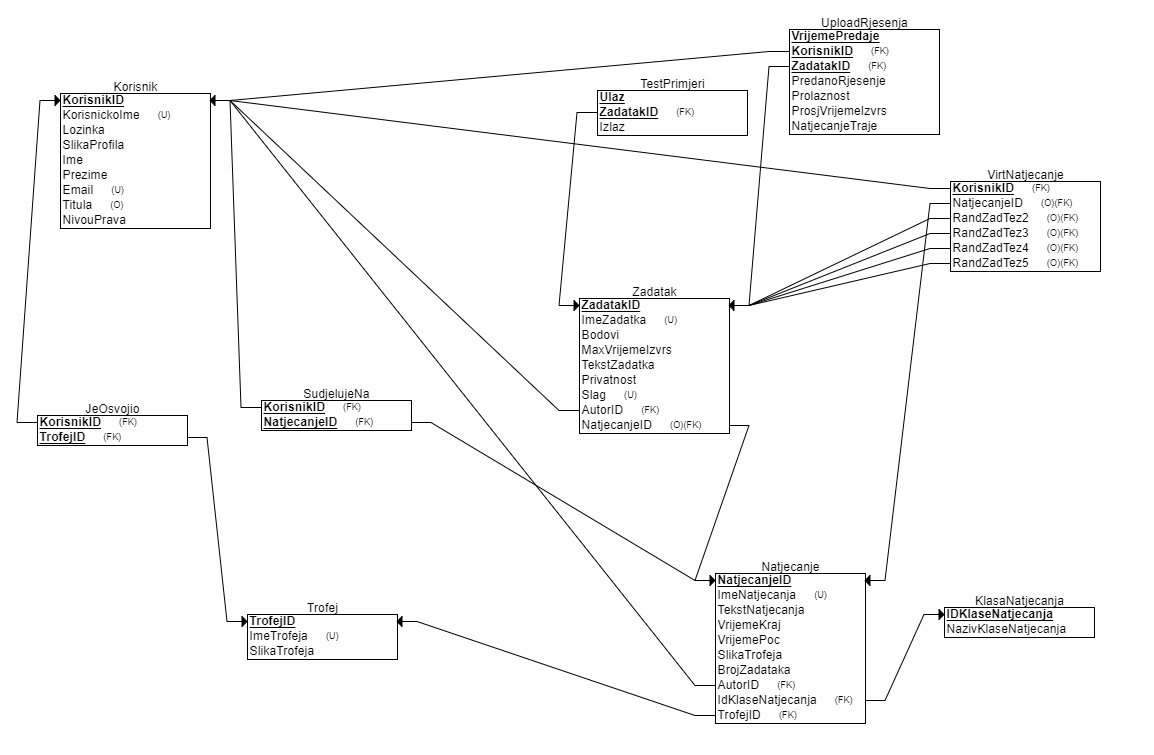
\includegraphics[width=\textwidth]{slike/RelacijskaShema.PNG} %veličina u odnosu na širinu linije
			\caption{E-R dijagram baze podataka}
			\label{fig:RelacijskaShema} %label mora biti drugaciji za svaku sliku
		\end{figure}
		
		\eject
			
			
		\section{Dijagram razreda}
			Na slici 4.2. vidimo osnovni model UML dijagrama koji prikazuje osnovne klase koje koristimo na backendu.
				
			Trenutni dijagram razreda opisuje izgled klasa i njihovih metoda koje će nam biti potrebne u projektu. 
			Trenutno pošto imamo registraciju, ulogiravanje i validaciju, koristimo samo klasu Korisnik te njene metode. 
			Imamo privatnu metodu koja se zove \verb*|__get_id()| preko koje dobivamo korisnikid iz baze podataka,
			zato što je to metoda koja dohvaća privatni ključ te ne želimo da korisnik ikad ima pristup tome.
			Tu metodu trenutno ne koristimo previše već će biti jako korisna kasnije u konekcijama s instancama ostalim
			klasa prilikom dobivanja informacija iz ostalih tablica baze podataka. Kao što se vidi, svaka klasa ima 
			konstruktor \verb*|__init__()| te primaju informacije koje su identične onima iz njihovih modela iz baze podataka.

			\begin{figure}[H]
				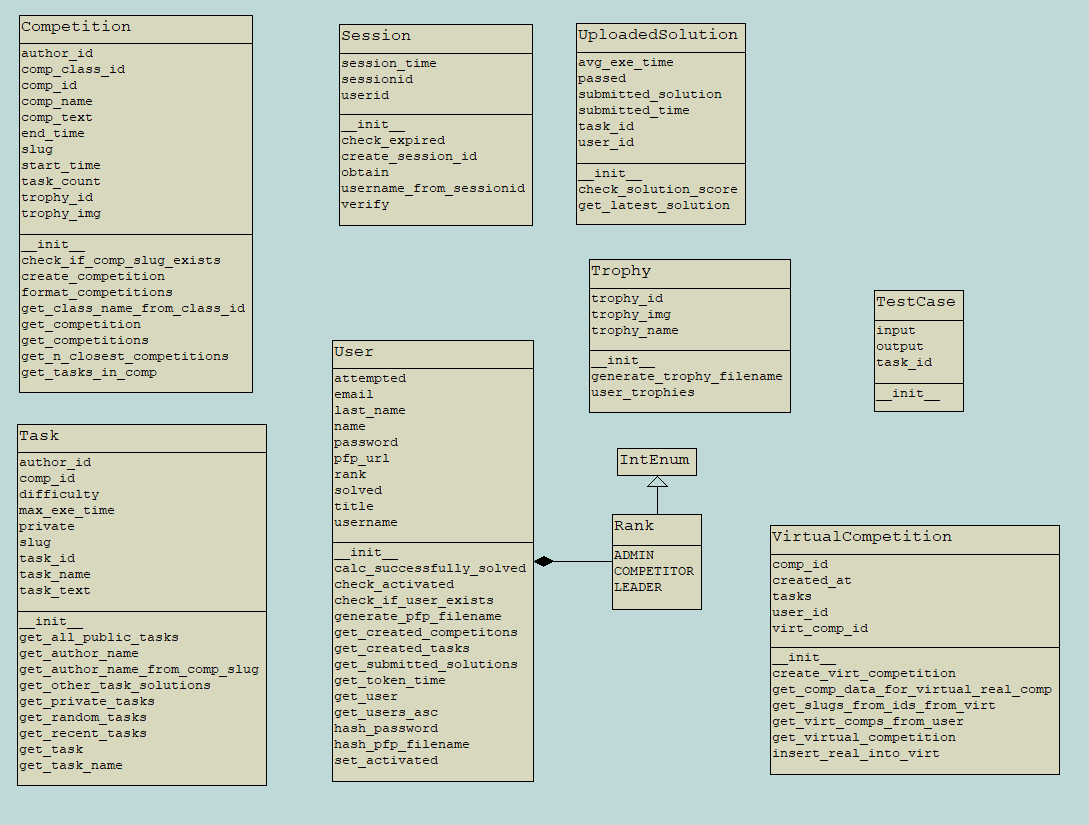
\includegraphics[width=\textwidth]{slike/DijagramRazreda.png} %veličina u odnosu na širinu linije
				\caption{Dijagram razreda}
				\label{fig:DijagramRazreda} %label mora biti drugaciji za svaku sliku
			\end{figure}	
			

			Budući da radimo u programskom jeziku Python, ne možemo lako prikazati Data Transfer objects.
			Međutim, prilikom registracije, sve informacije koje dobivamo s frontenda prosljeđujemo u konstruktor
			Korisnik. Kasnije, prilikom login-a, preko korisničkog imena dobivamo podatke iz baze te izrađujemo instancu Korisnik.
			S tim Korisnikom možemo baratati pomoću njegovih podataka. Tražimo iz baze podataka je li aktiviran te odgovara li
			hash unesene lozinke hashu lozinke koja je spremljena u bazu podataka, tj. u instanci Korisnik.

			Naša klasa Korisnik se zapravo referira i na voditelja i na administratora. Oni svi imaju identične podatke te duplikacija koda
			nije potrebna. Velika razlika je samo u njihovom podatku NivouPrava o kojem će ovisiti kakve ovlasti na stranici ima.
			To će također biti funkcija koju će biti privatna. Voditelj će za razliku od natjecatelja imati pristup stranicama
			za  kreiranje zadataka te stvaranju natjecanja. Administrator će uz to sve moći uređivati ovlasti svih korisnika te će pomoću toga imati mogućnost potvrditi voditelja što će biti na posebnoj stranici.



				\eject
			
			\textbf{\textit{dio 2. revizije}}\\			
			
			\textit{Prilikom druge predaje projekta dijagram razreda i opisi moraju odgovarati stvarnom stanju implementacije}
			
			
			
			\eject
		
		\section{Dijagram stanja}
			
		
			\textbf{\textit{dio 2. revizije}}\\
			
			\textit{Potrebno je priložiti dijagram stanja i opisati ga. Dovoljan je jedan dijagram stanja koji prikazuje \textbf{značajan dio funkcionalnosti} sustava. Na primjer, stanja korisničkog sučelja i tijek korištenja neke ključne funkcionalnosti jesu značajan dio sustava, a registracija i prijava nisu. }
			
			
			\eject 
		
		\section{Dijagram aktivnosti}
			
			\textbf{\textit{dio 2. revizije}}\\
			
			 \textit{Potrebno je priložiti dijagram aktivnosti s pripadajućim opisom. Dijagram aktivnosti treba prikazivati značajan dio sustava.}
			
			\eject
		\section{Dijagram komponenti}
		
			\textbf{\textit{dio 2. revizije}}\\
		
			 \textit{Potrebno je priložiti dijagram komponenti s pripadajućim opisom. Dijagram komponenti treba prikazivati strukturu cijele aplikacije.}
	\chapter{Implementacija i korisničko sučelje}
		
		\section{Korištene tehnologije i alati}
		
			Komunikacija u timu realizirana je korištenjem aplikacija \underline{WhatsApp}\footnote{https://www.whatsapp.com/} i \underline{Discord} \footnote{https://discord.com/}. Za izradu	UML dijagrama korišten je alat \underline{Astah UML} \footnote{https://astah.net/products/astah-uml/}  , a kao sustav za upravljanje izvornim kodom \underline{Git}\footnote{https://git-scm.com/}. Udaljeni repozitorij projekta je dostupan na web platformi \underline{GitLab} \footnote{https://gitlab.com/} .
			Kao razvojno okruženje korišten je \underline{Visual Studio Code}\footnote{https://code.visualstudio.com/}. Prvenstveno se koristi kao uređivač teksta pri razvoju računalnih programa za operacijski sustav Windows, kao i za web-stranice, web-aplikacije, web-usluge i mobilne aplikacije. Aplikacija je napisana koristeći radni okvir \underline{Flask}\footnote{https://flask.palletsprojects.com/en/2.0.x/} i web poslužitelj \underline{Gunicorn}\footnote{https://gunicorn.org/} u jeziku \underline{Python 3.8}. \footnote{https://www.python.org/} za izradu backenda. Za izradu frontenda su se koristili razvojni okvir \underline{React}\footnote{https://reactjs.org/} i jezik \underline{JavaScript}\footnote{https://www.javascript.com/}. React, takoder poznat kao React.js ili ReactJS, je biblioteka u JavaScriptu za izgradnju korisničkih sučelja. React se najčešće koristi kao osnova	u razvoju web ili mobilnih aplikacija. Složene aplikacije u Reactu obično zahtijevaju korištenje dodatnih biblioteka za interakciju s API-jem. Web poslužitelj Gunicorn nadograđuje radni okvir Flask kako bi mogao posluživati više zahtjeva u isto vrijeme. Naša cijela infrastruktura se nalazi u oblaku na privatnom VPS poslužitelju, poslužuje zahtjeve pomoću \underline{NGINX}\footnote{https://nginx.org/en/} web poslužitelja na linux  ubuntu sustavu.
			Mrežna potpora našoj arhitekturi je \underline{CloudFlare} \footnote{https://www.cloudflare.com/} koja nam nudi usluge poput predmemorije (engl. cache) i DDoS zaštite. Bitan dio naše infrastrukture je baza podataka realizirana kroz \underline{PostgreSQL RDBMS}\footnote{https://www.postgresql.org/}.
			
			
			\eject 
		
	
		\section{Ispitivanje programskog rješenja}
		
			 Svi testovi izvršeni su pomoću skripte u Pythonu koristeći Selenium WebDriver i pytest. Ispitivanje se radilo po obrascima uporabe kako bi se provjerila osnovna funkcionalnost sustava, ali i nasumičnim kretanjima po aplikaciji kako bi se pronašle neočekivane greške(”bugovi”) ili nepredviđena ponašanja. Svaki dio sustava je ispitan, no zbog jednostavnosti u dokumentaciji će biti prikazan samo dio ispitivanja.
	
			
			\subsection{Ispitivanje komponenti}
			\textbf{Ispitni slučajevi}: \newline
			Provedeno je ispitivanje jedinca za 6 ispitnih slučajeva. Ti su slučajevi redom:
			\begin{enumerate}
				\item Konekcija na bazu podataka
				\item Provjera postojanja korisnika
				\item Dohvaćanje imena klase natjecanja
				\item Dohvaćanje zadatka
				\item Dohvaćanje imena zadatka
				\item Dohvaćanje virtualnog natjecanja
			\end{enumerate}
			
			\noindent  \textbf{Očekivani rezultati}: 
			\begin{enumerate}
				\item Uspješna spajanje s bazom podataka
				\item Uspješno/Neuspješno postojanje korisnika ovisno o parametrima
				\item Uspješno dohvaćanje imena klase natjecanja
				\item Uspješno dohvaćanje zadatka
				\item Uspješno dohvaćanje punog imena zadatka
				\item Uspješno dohvaćanje virtualnog natjecanja
			\end{enumerate}
			
			\begin{figure}[H]
				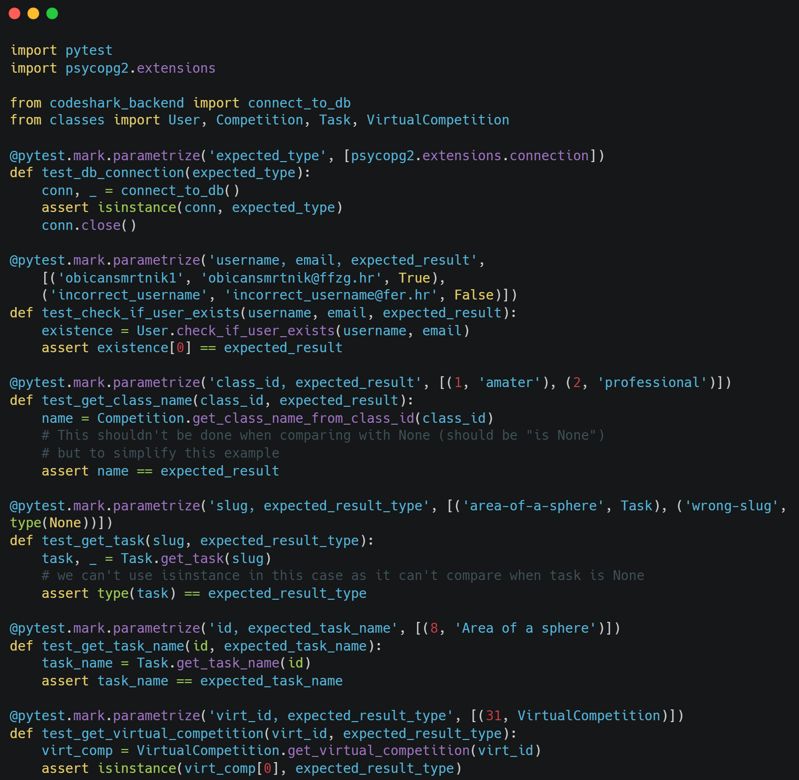
\includegraphics[width=\textwidth]{slike/IspitivanjeKomponenti.png} %veličina u odnosu na širinu linije
				\caption{Ispitivanje komponenti}
				\label{fig:IspitivanjeKomponenti} %label mora biti drugaciji za svaku sliku
			\end{figure}
		
			\begin{figure}[H]
				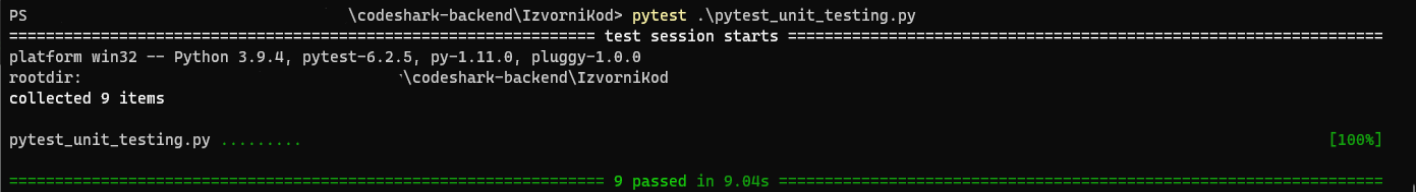
\includegraphics[width=\textwidth]{slike/IspitivanjeKomponentiRez.png} %veličina u odnosu na širinu linije
				\caption{Rezultat ispitivanja komponenti}
				\label{fig:IspitivanjeKomponentiRez} %label mora biti drugaciji za svaku sliku
			\end{figure}
		
			\noindent \textbf{Rezultat}: 
			\newline 
			Svi očekivani rezultati su zadovoljeni.
			
			
			
			\subsection{Ispitivanje sustava}
			\textbf{Ispitni slučajevi}: \newline
			Provedeno je ispitivanje jedinca za 6 ispitnih slučajeva. Ti su slučajevi redom:
			\begin{enumerate}
				\item Dohvaćanje početne stranice
				\item Dohvaćanje popisa korisnika od strane neregistriranog korisnika
				\item Dohvaćanje popisa korisnika od strane registriranog korisnika
				\item Testiranje prijave
				\item Dohvaćanje profilne stranice od strane neregistriranog korisnika
				\item Dohvaćanje profilne stranice od strane registriranog korisnika
			\end{enumerate}
			
			\noindent  \textbf{Očekivani rezultati}: 
			\begin{enumerate}
				\item Stranica je uspješno dohvaćena
				\item Stranica preusmjeruje na stranicu prijave
				\item Stranica je uspješno dohvaćena
				\item Uspješna/Neuspješna prijava ovisno o parametrima
				\item Stranica preusmjeruje na stranicu prijave
				\item Stranica je uspješno dohvaćena
			\end{enumerate}
			
			\begin{figure}[H]
				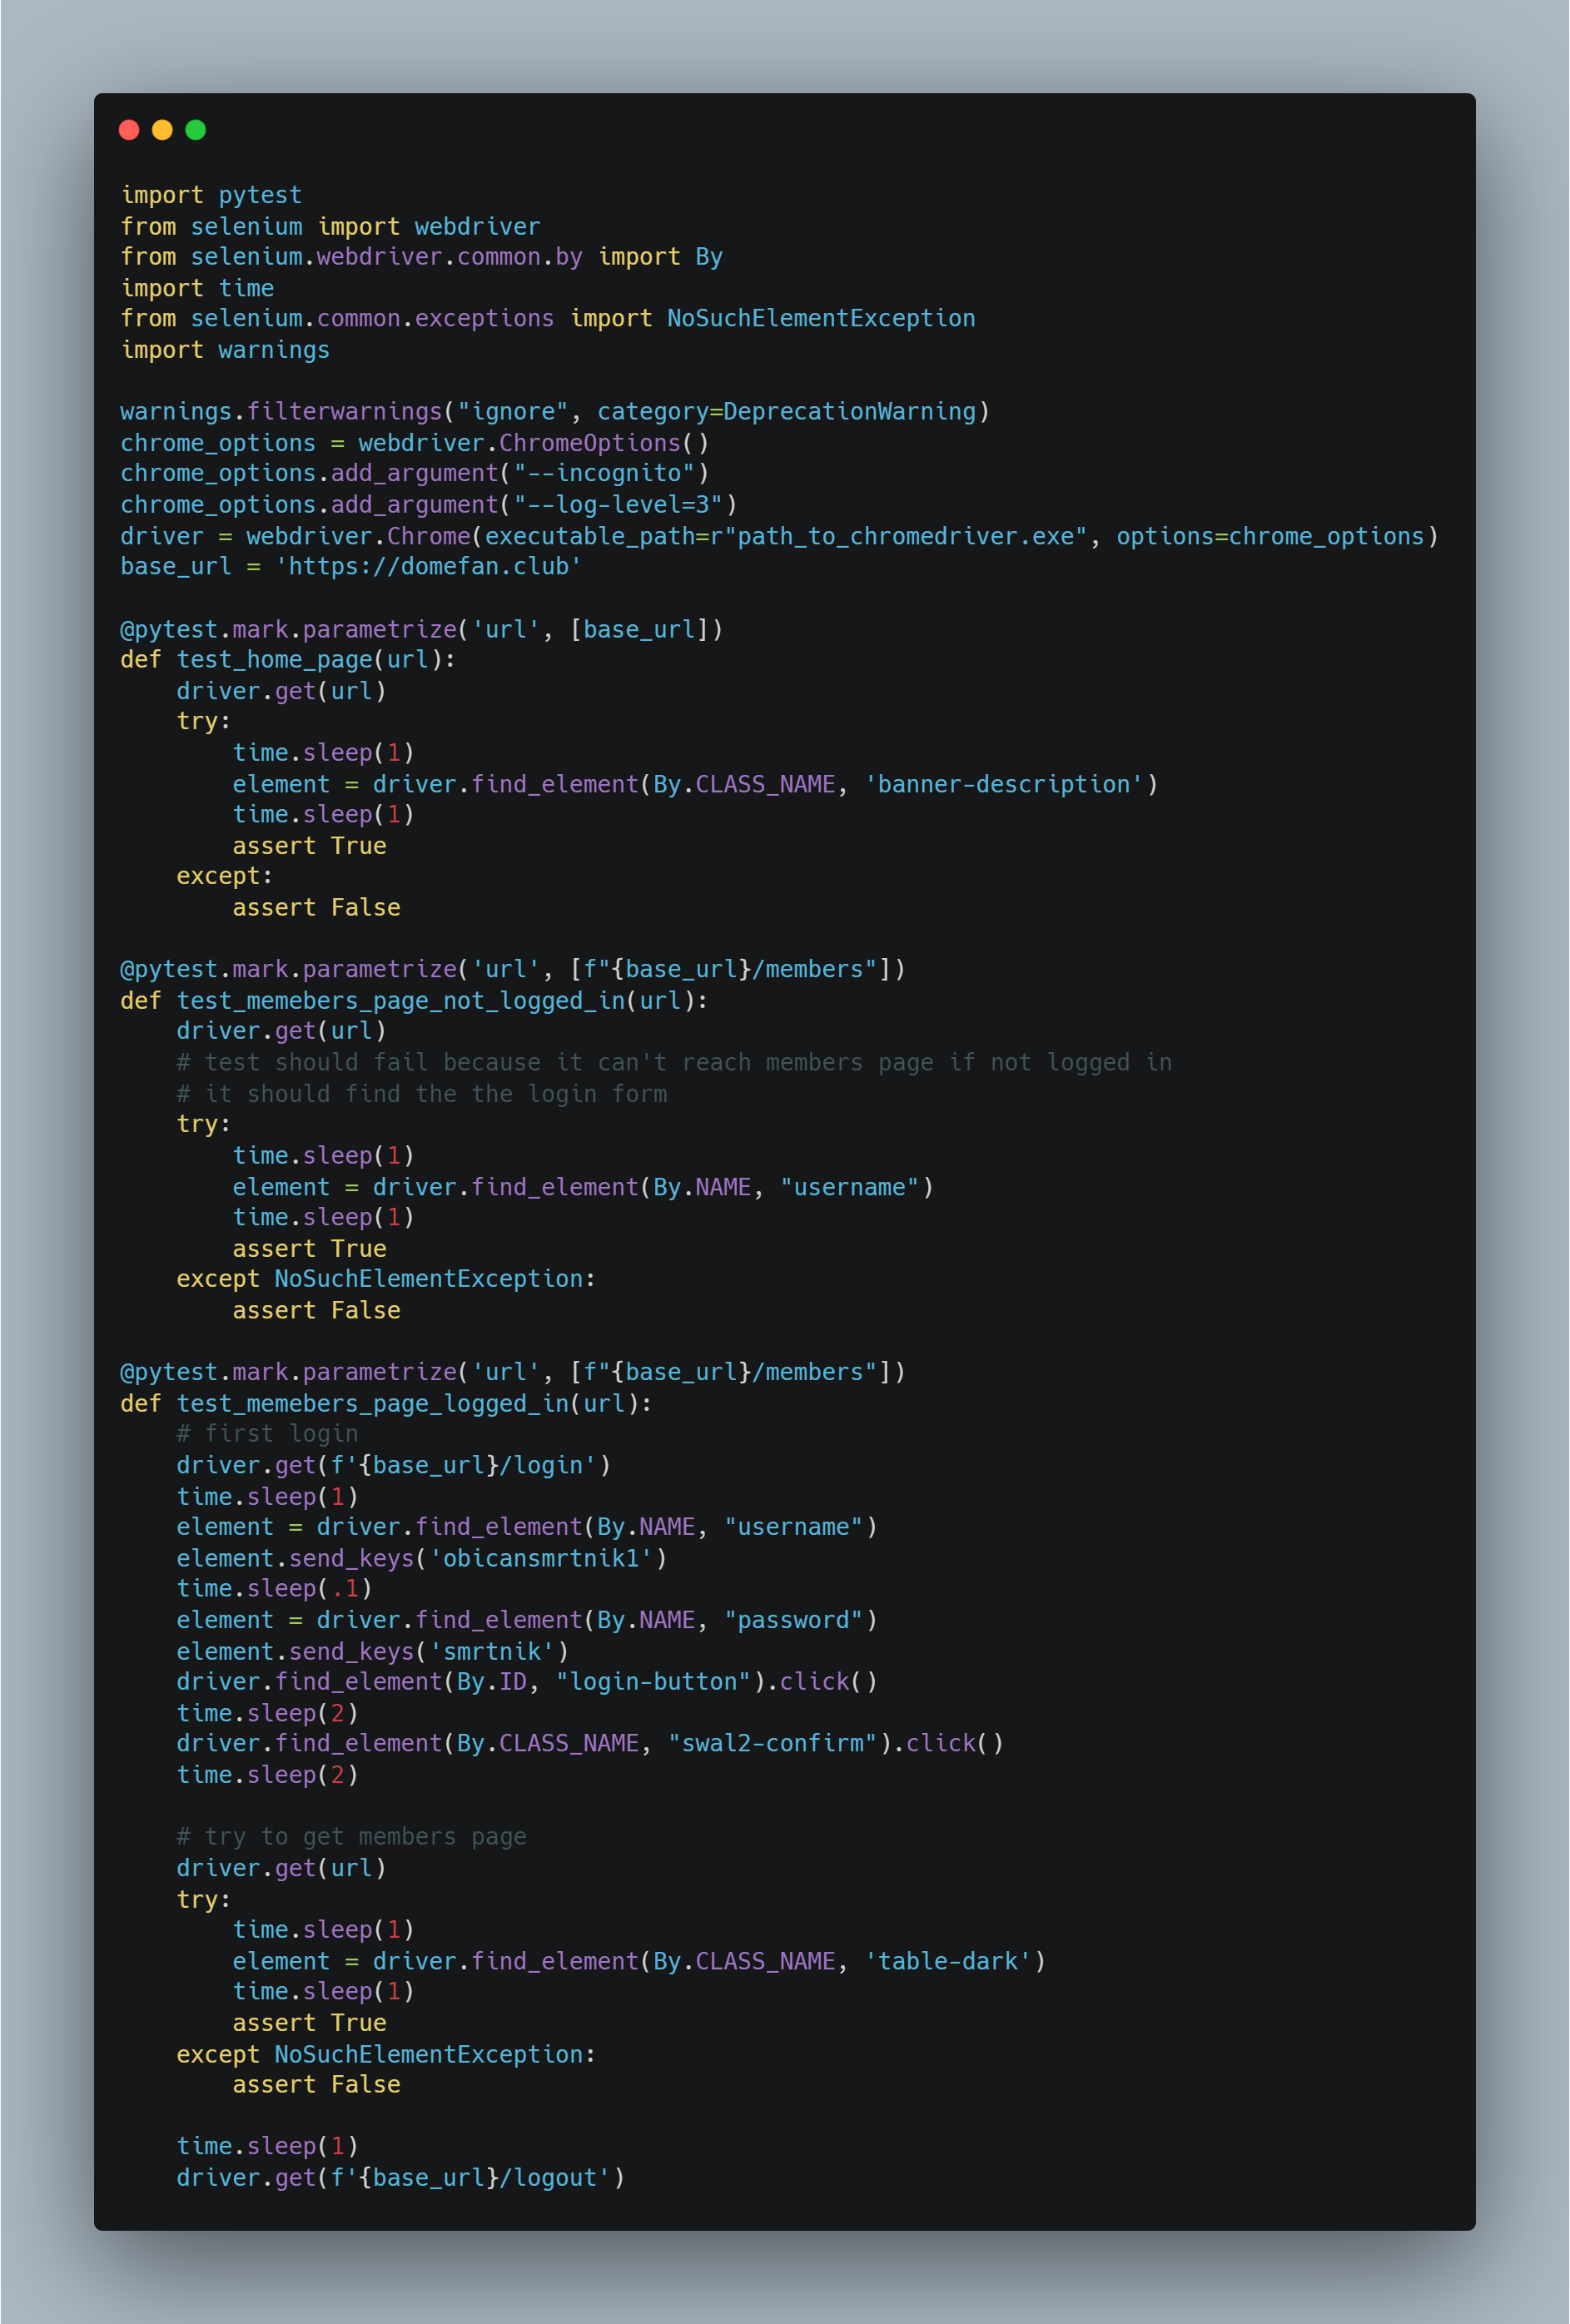
\includegraphics[width=\textwidth]{slike/IspitivanjeSustavaPrviDio.png} %veličina u odnosu na širinu linije
				\caption{Ispitivanje sustava prvi dio}
				\label{fig:IspitivanjeSustavaPrviDio} %label mora biti drugaciji za svaku sliku
			\end{figure}
			\begin{figure}[H]
				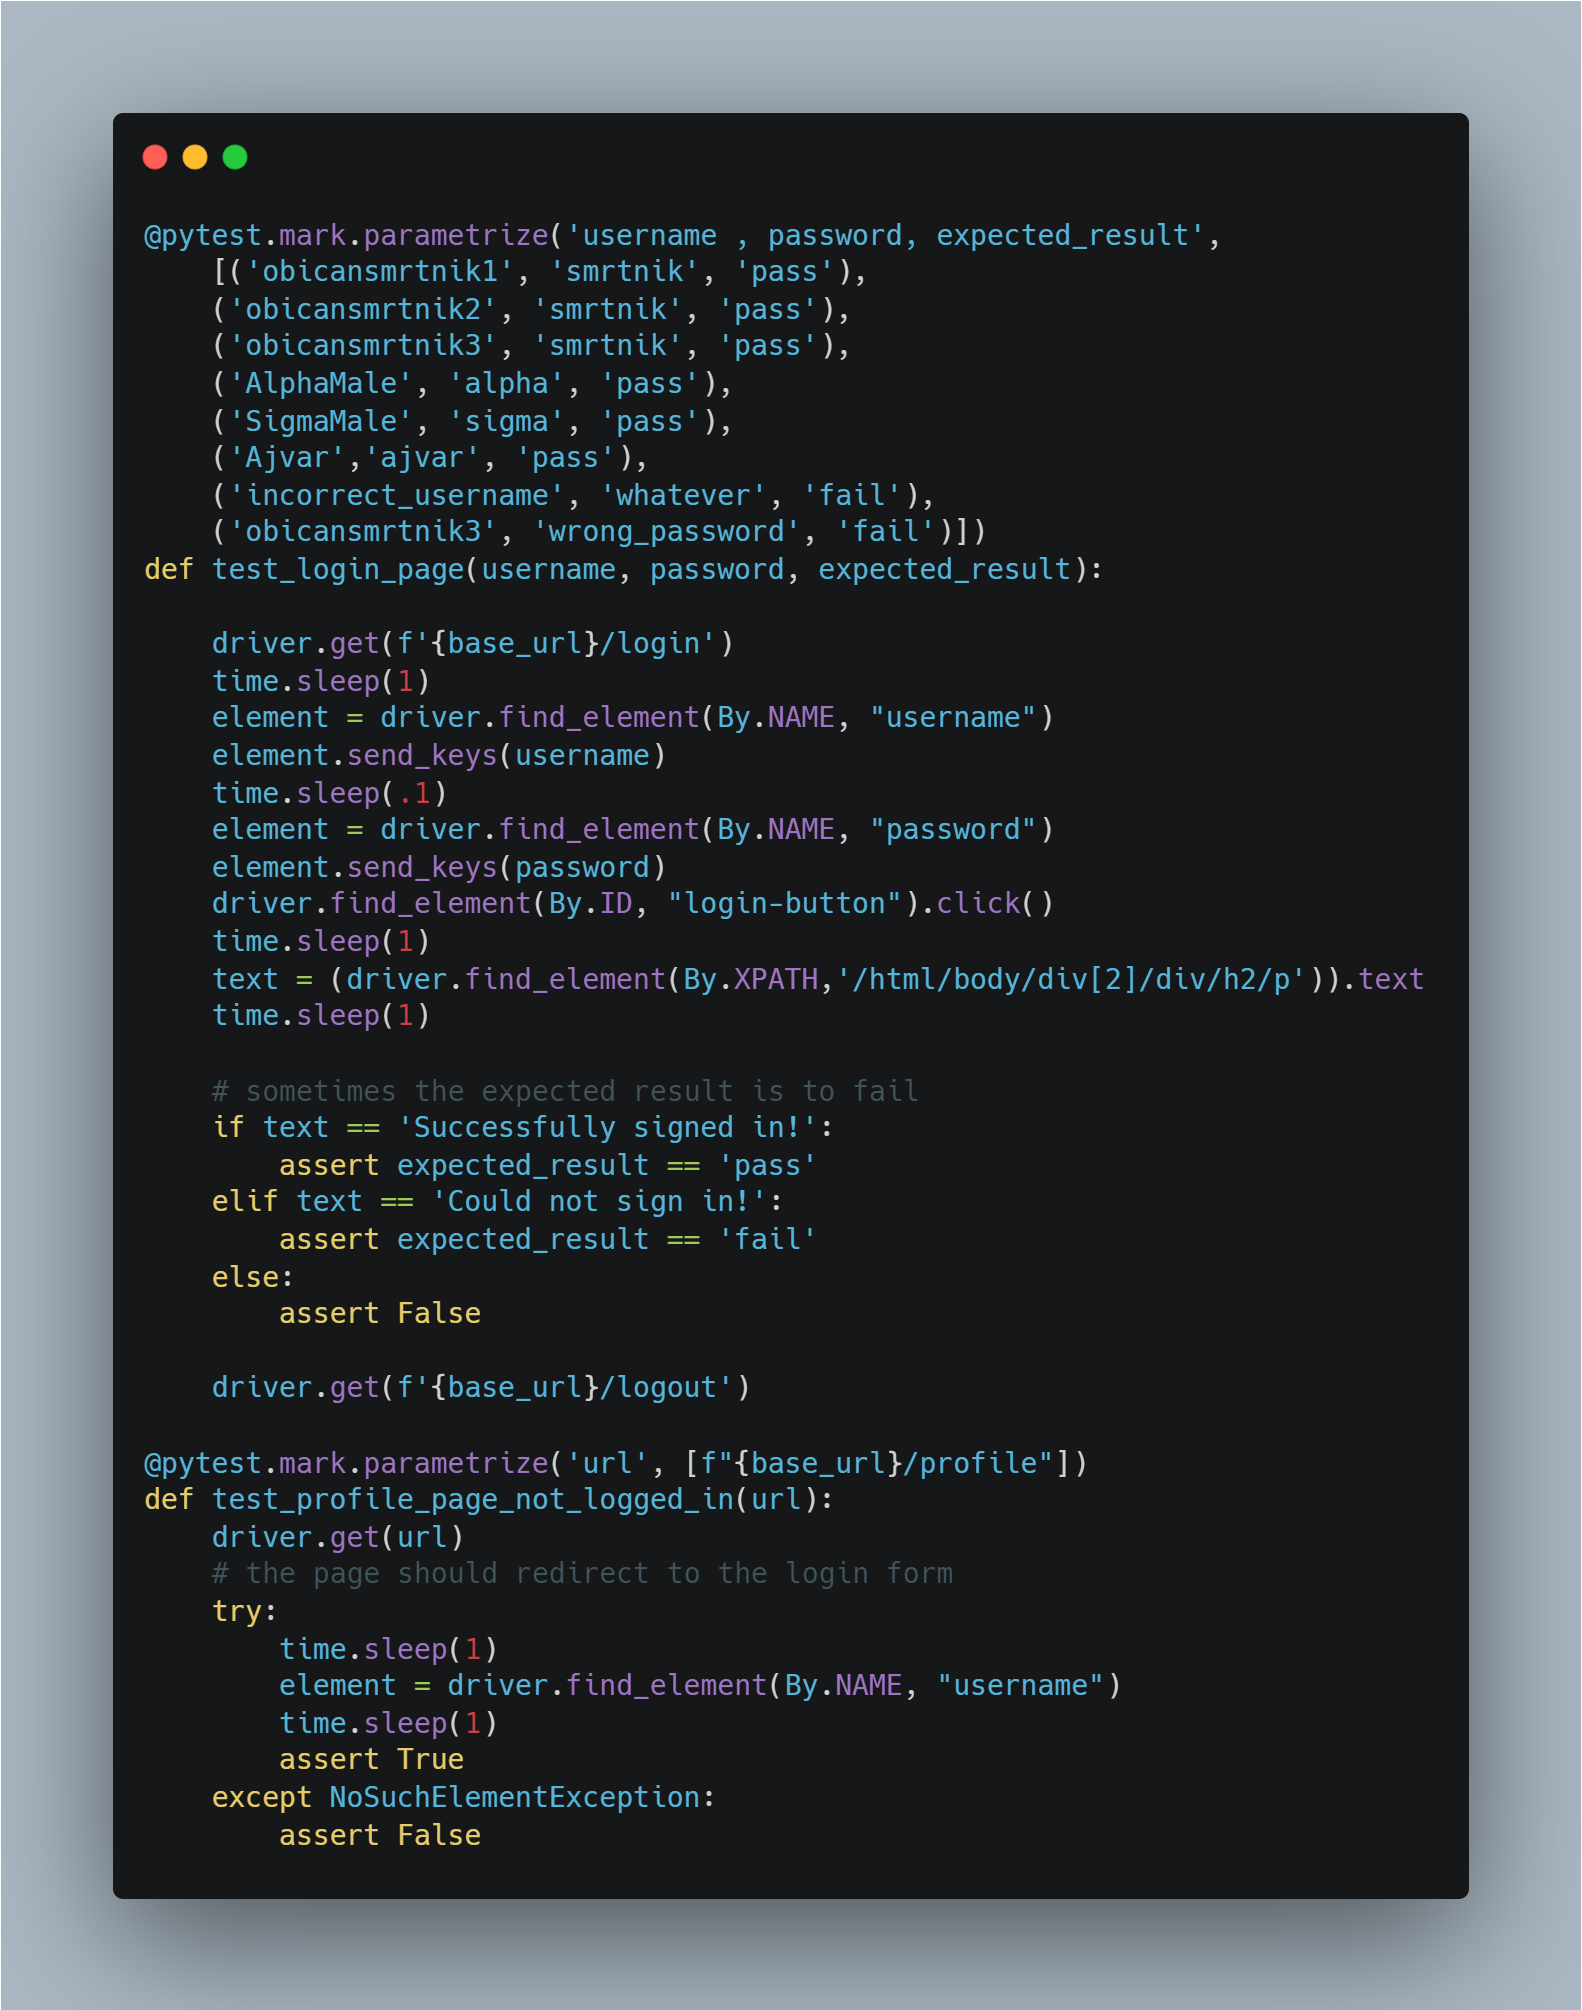
\includegraphics[width=\textwidth]{slike/IspitivanjeSustavaDrugiDio.png} %veličina u odnosu na širinu linije
				\caption{Ispitivanje sustava drugi dio}
				\label{fig:IspitivanjeSustavaDrugiDio} %label mora biti drugaciji za svaku sliku
			\end{figure}
		
			\begin{figure}[H]
				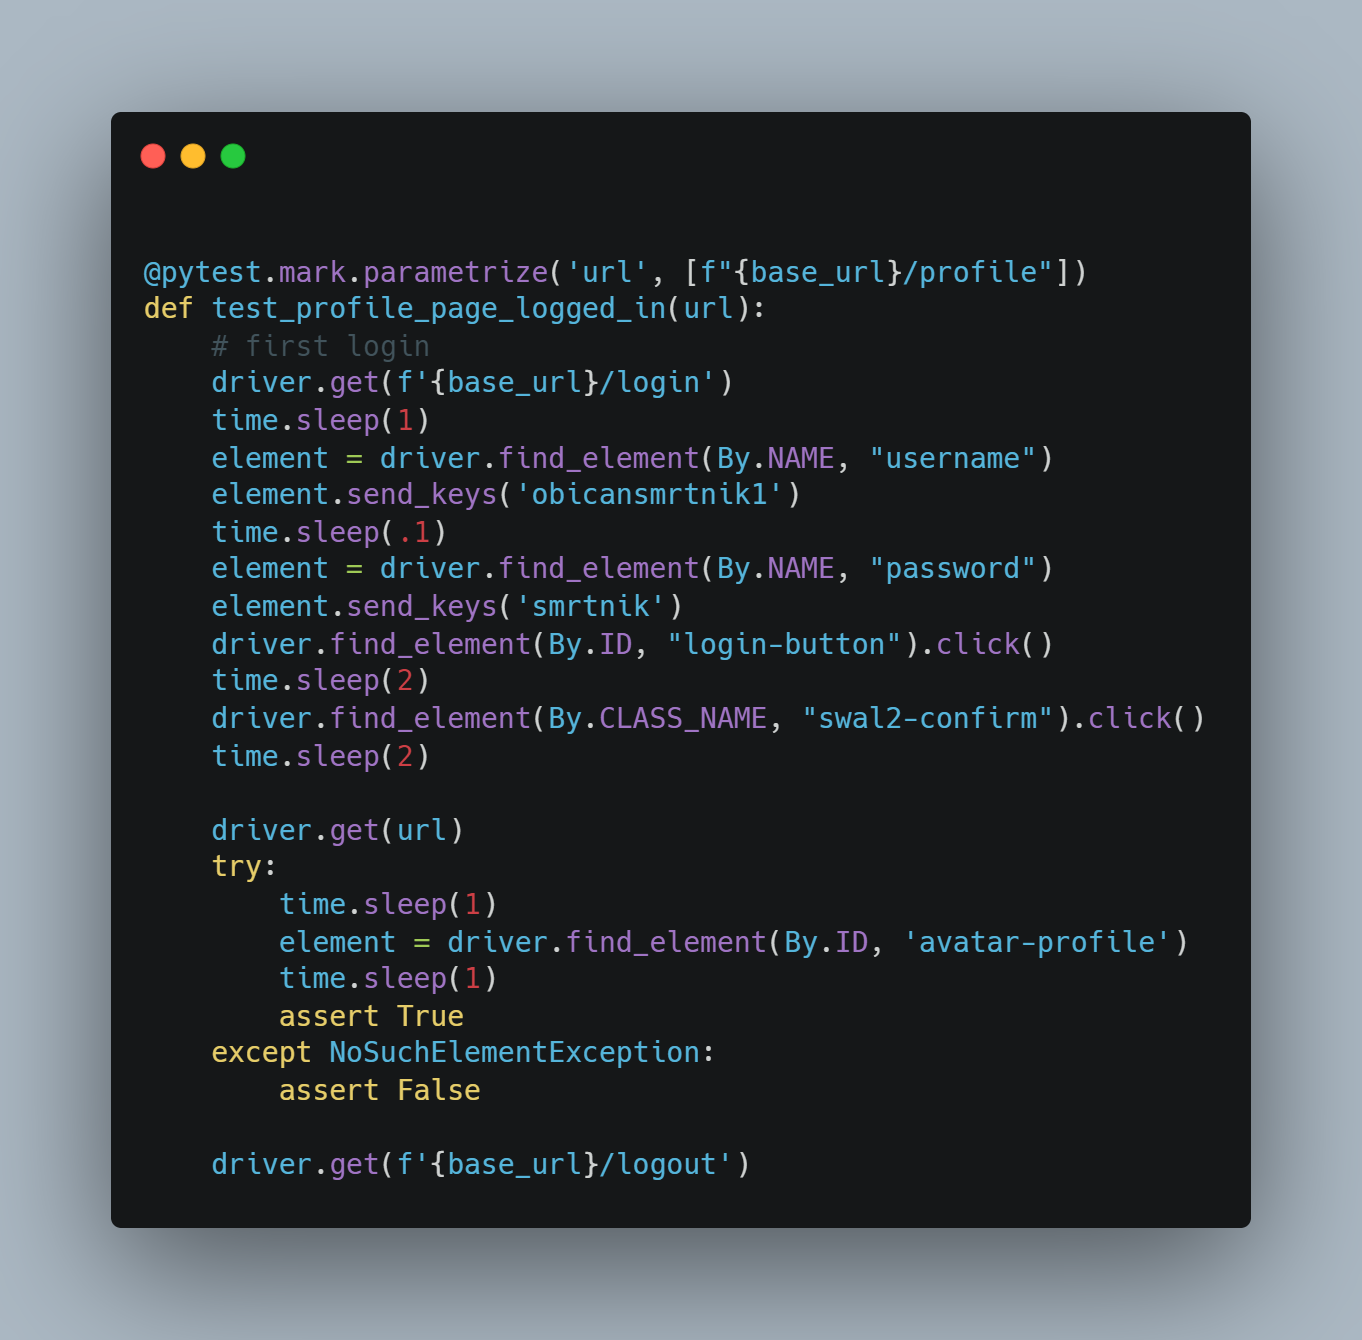
\includegraphics[width=\textwidth]{slike/IspitivanjeSustavaTreciDio.png} %veličina u odnosu na širinu linije
				\caption{Ispitivanje sustava treći dio}
				\label{fig:IspitivanjeSustavaTrećoDio} %label mora biti drugaciji za svaku sliku
			\end{figure}
			
			\begin{figure}[H]
				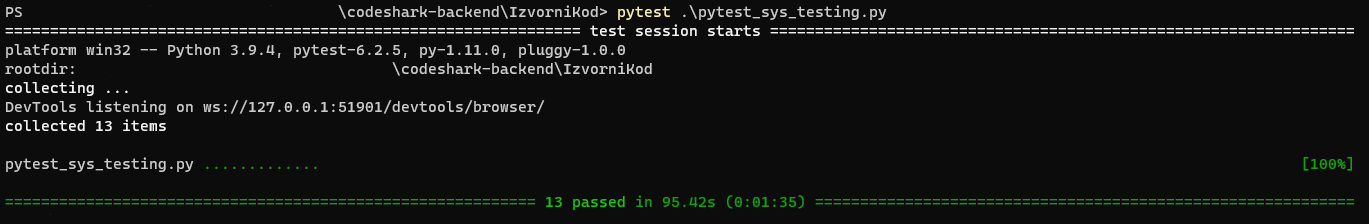
\includegraphics[width=\textwidth]{slike/IspitivanjeSustavaRez.png} %veličina u odnosu na širinu linije
				\caption{Rezultat ispitivanja sustava}
				\label{fig:IspitivanjeSustavaRez} %label mora biti drugaciji za svaku sliku
			\end{figure}
			
			\noindent  \textbf{Rezultat}: \newline
			Svi očekivani rezultati su zadovoljeni.
			 
			 
			
			\eject 
		
		
		\section{Dijagram razmještaja}
			
			Dijagrami razmještaja opisuju topologiju sklopovlja i programsku potporu koja se koristi u implementaciji sustava u njegovom radnom okruženju. Na poslužiteljskom računalu se nalaze web poslužitelj i poslužitelj baze podataka. Klijenti koriste web preglednik kako bi pristupili web aplikaciji. Sustav je baziran na arhitekturi ”klijent – poslužitelj”, a komunikacija između računala korisnika (klijent, zaposlenik, vlasnik, administrator) i poslužitelja odvija se preko HTTPS veze.
			
			
			\begin{figure}[H]
				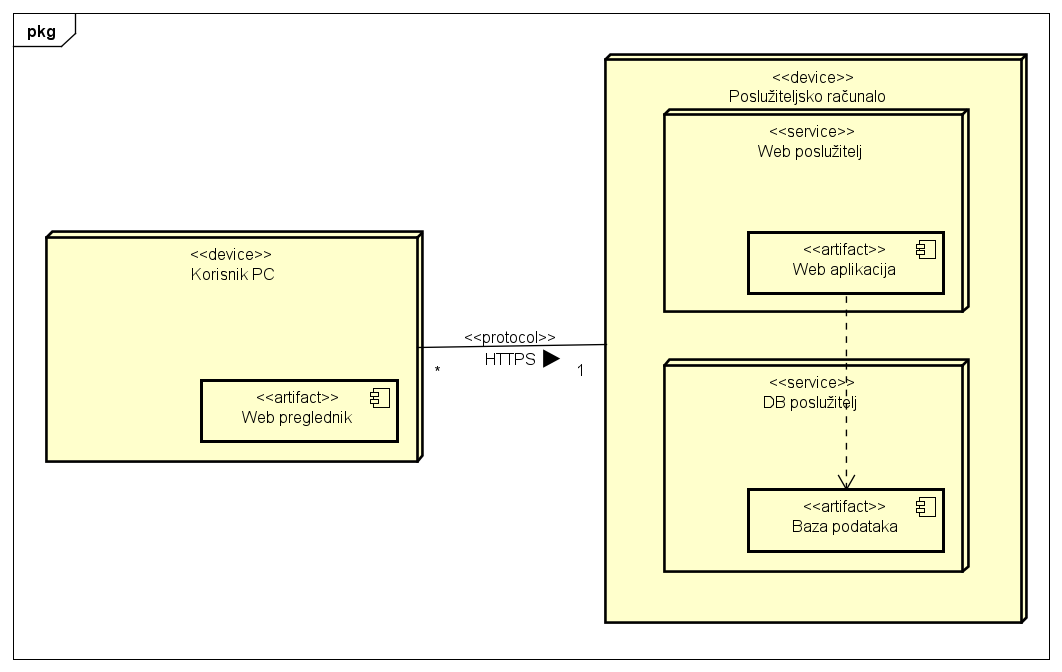
\includegraphics[width=\textwidth]{slike/DijagramRazmjestaja.png} %veličina u odnosu na širinu linije
				\caption{Dijagram Razmještaja}
				\label{fig:DijagramRazmještaja} %label mora biti drugaciji za svaku sliku
			\end{figure}
			
			\eject 
		
		\section{Upute za puštanje u pogon}
		
			\textbf{Instalacija poslužitelja baze podataka}\\
		
			 Potrebno je preuzeti Oracle MySql bazu podataka (za operacijski sustav Windows).
			 Poželjno je skinuti čitav paket Oracle Workbench. Nakon toga je potrebno provesti standardnu instalaciju s postavljanjem korisnika.
			
			
			 \textit{Dovršenu aplikaciju potrebno je pokrenuti na javno dostupnom poslužitelju. Studentima se preporuča korištenje neke od sljedećih besplatnih usluga: \href{https://aws.amazon.com/}{Amazon AWS}, \href{https://azure.microsoft.com/en-us/}{Microsoft Azure} ili \href{https://www.heroku.com/}{Heroku}. Mobilne aplikacije trebaju biti objavljene na F-Droid, Google Play ili Amazon App trgovini.}
			
			
			\eject 
	\chapter{Zaključak i budući rad}
		
		Zadatak naše grupe bio je razvoj web aplikacije koja omogućuje provjeru riješenih programskih zadataka i sudjelovanje u natjecanjima. Nakon 17 tjedana rada u timu i razvoja, ostvarili smo zadani cilj. Rad na projektu se vršio kroz dvije faze. 
		\newline \hspace*{12pt}
		Prva faza projekta je započela okupljanjem tima za razvoj aplikacije, dodjelu projektnog zadatka, koncipiranje izvedbe projektnog zadatka te dokumentiranju zahtjeva. Kvalitetna komunikacija u prvoj fazi uvelike je olakšala daljnji rad pri realizaciji osmišljenog sustava. Rani fokus na izradu vizualnih prikaza svih idejnih rješenja zadanog zadatka je omogućila članovima projekta lakšu koordinaciju i smanjila je pojave raznih nedoumica koje su se mogle pojaviti.
		\newline \hspace*{12pt}
		Druga faza projekta, iako nešto kraća od prve, bila je puno intenzivnija po pitanju samostalnog rada članova. Manjak iskustva članova u izradi sličnih implementacijskih rješenja primorao je članove na samostalno učenje odabranih alata i programskih jezika kako bi ispunili dogovorene ciljeve. Nasreću, projektni tim je imao ljude koji su vještiji s odabranim tehnologijama, pa se proces učenja kod ostalih znatno ubrzao. Osim implementacije svih zahtjeva, dio druge faze se isto fokusirao na izvedbe UML dijagrama i popratne dokumentacije kako bi budućim korisnicima bilo lakše koristiti ili vršiti preinake na sustavu.
		\newline \hspace*{12pt}
		Komunikacija medu članovima tima je bila pretežito uživo kako bi dočarali osjećaj timskog rada i zajedništva. Tome su naravno pomogli redovni "Team-buildinzi" svakakvih vrsta. Ostala komunikacije se vršila putem WhatsAppa i Discorda. Jedno od mogućih proširenja sustava je uvođenje funkcije slanje poruka između korisnika te podizanje foruma što bi uvelike proširilo ciljani fokus na unapređenju pojedinaca kroz rad.
		\newline \hspace*{12pt}
		Sudjelovanje na ovakvom projektu bilo je vrijedno iskustvo svim članovima
		tima jer je to većini prvi ozbiljniji grupni projekt na kojem se moralo u kratkom roku intenzivno raditi. Također se iskusila važnost komunikacije i koordiniranosti između članova tima. Cijeli tim je zadovoljan postignutim i smatra da će ovakvo iskustvo biti vrlo korisno kroz daljnje fakultativno i poslovno obrazovanje. 
		
		
		\eject 
	\chapter*{Popis literature}
		\addcontentsline{toc}{chapter}{Popis literature}
	 	
 		\textbf{\textit{Kontinuirano osvježavanje}}
	
		\textit{Popisati sve reference i literaturu koja je pomogla pri ostvarivanju projekta.}
		
		
		\begin{enumerate}
			
			
			\item  Programsko inženjerstvo, FER ZEMRIS, \url{http://www.fer.hr/predmet/proinz}
			
			\item  I. Sommerville, "Software engineering", 8th ed, Addison Wesley, 2007.
			
			\item  T.C.Lethbridge, R.Langaniere, "Object-Oriented Software Engineering", 2nd ed. McGraw-Hill, 2005.
			
			\item  I. Marsic, Software engineering book``, Department of Electrical and Computer Engineering, Rutgers University, \url{http://www.ece.rutgers.edu/~marsic/books/SE}
			
			\item  The Unified Modeling Language, \url{https://www.uml-diagrams.org/}
			
			\item  Astah Community, \url{http://astah.net/editions/uml-new}
		\end{enumerate}
		
		 
	
	
	\begingroup
	\renewcommand*\listfigurename{Indeks slika i dijagrama}
	%\renewcommand*\listtablename{Indeks tablica}
	%\let\clearpage\relax
	\listoffigures
	%\vspace{10mm}
	%\listoftables
	\endgroup
	\addcontentsline{toc}{chapter}{Indeks slika i dijagrama}


	
	\eject 
		
	\chapter*{Dodatak: Prikaz aktivnosti grupe}
		\addcontentsline{toc}{chapter}{Dodatak: Prikaz aktivnosti grupe}
		
		\section*{Dnevnik sastajanja}
		
		
		
		\begin{packed_enum}
			\item  sastanak
			
			\item[] \begin{packed_item}
				\item Datum: 12. listopada 2021. 
				\item Prisustvovali: M.Damjanić, F.Tomljenović, I.Jeržabek, A.Griparić, R.Mihalić
				\item Teme sastanka:
				\begin{packed_item}
					\item  Moguće alternativne ideje za projekt
					\item  Početne ideje za tehnologije
				\end{packed_item}
			\end{packed_item}
			
			\item  sastanak
			\item[] \begin{packed_item}
				\item Datum: 14. listopada 2021. 
				\item Prisustvovali: M.Damjanić, F.Tomljenović, I.Jeržabek, A.Griparić, R.Mihalić, L.Maros, F.Jelavić
				\item Teme sastanka:
				\begin{packed_item}
					\item  Dogovorene korištene tehnologije
				\end{packed_item}
			\end{packed_item}
		
			\item  sastanak
			\item[] \begin{packed_item}
				\item Datum: 28. listopada 2021. 
				\item Prisustvovali: M.Damjanić, F.Tomljenović, I.Jeržabek, A.Griparić, R.Mihalić, L.Maros, F.Jelavić
				\item Teme sastanka:
				\begin{packed_item}
					\item  Predložen koncept cijelog projekta
					\item  Podjela posla po članovima za 1.ciklus
				\end{packed_item}
			\end{packed_item}
		
			\item  sastanak
			\item[] \begin{packed_item}
				\item Datum: 12. studeni 2021. 
				\item Prisustvovali: M.Damjanić, F.Tomljenović, I.Jeržabek, A.Griparić, R.Mihalić, L.Maros, F.Jelavić
				\item Teme sastanka:
				\begin{packed_item}
					\item  Jeržabek je održao predavanje o Reactu
					\item  Dane upute o spajanju na bazu i pisanju dokumentacije
				\end{packed_item}
			\end{packed_item}
			
			\eject
			\item  sastanak
			\item[] \begin{packed_item}
				\item Datum: 17. studeni 2021. 
				\item Prisustvovali: M.Damjanić, I.Jeržabek, A.Griparić, R.Mihalić
				\item Teme sastanka:
				\begin{packed_item}
					\item   Sastanak s asistentom i demosom - evaluacija dosadašnjeg rada
				\end{packed_item}
			\end{packed_item}
		
			\item  sastanak
			\item[] \begin{packed_item}
				\item Datum: 8. prosinca 2021. 
				\item Prisustvovali: M.Damjanić, F.Tomljenović, I.Jeržabek, A.Griparić, R.Mihalić, L.Maros, F.Jelavić
				\item Teme sastanka:
				\begin{packed_item}
					\item  Prolaženje kroz svih dijelova projekta sa svim članovima
				\end{packed_item}
			\end{packed_item}
		
			\item  sastanak
			\item[] \begin{packed_item}
				\item Datum: 16. prosinca 2021. 
				\item Prisustvovali: M.Damjanić, F.Tomljenović, I.Jeržabek, A.Griparić, R.Mihalić, L.Maros
				\item Teme sastanka:
				\begin{packed_item}
					\item  Dogovorene raspodjela poslova za 2.ciklus
				\end{packed_item}
			\end{packed_item}
		
			\item  sastanak
			\item[] \begin{packed_item}
				\item Datum: 21. prosinac 2021. 
				\item Prisustvovali: F.Tomljenović, I.Jeržabek, A.Griparić, R.Mihalić, L.Maros
				\item Teme sastanka:
				\begin{packed_item}
					\item   sastanak s asistentom i demosom - demonstracija alfa inačice
				\end{packed_item}
			\end{packed_item}
		
			\item  sastanak
			\item[] \begin{packed_item}
				\item Datum: 13. siječnja 2022. 
				\item Prisustvovali: M.Damjanić, I.Jeržabek, R.Mihalić
				\item Teme sastanka:
				\begin{packed_item}
					\item  sastanak s asistentom za zadnje implementacije i izvođenje buduće prezentacije
				\end{packed_item}
			\end{packed_item}			
			%
			
		\end{packed_enum}
		
		\eject
		\section*{Tablica aktivnosti}
		
			

			\begin{longtblr}[
					label=none,
				]{
					vlines,hlines,
					width = \textwidth,
					colspec={X[7, l]X[1, c]X[1, c]X[1, c]X[1, c]X[1, c]X[1, c]X[1, c]}, 
					vline{1} = {1}{text=\clap{}},
					hline{1} = {1}{text=\clap{}},
					rowhead = 1,
				} 
				\multicolumn{1}{c|}{} & \multicolumn{1}{c|}{\rotatebox{90}{\textbf{Marko Damjanić}}} & \multicolumn{1}{c|}{\rotatebox{90}{\textbf{Ivan Jeržabek}}} &	\multicolumn{1}{c|}{\rotatebox{90}{\textbf{Roko Mihalić}}} & \multicolumn{1}{c|}{\rotatebox{90}{\textbf{Fran Tomljenović}}} &	\multicolumn{1}{c|}{\rotatebox{90}{\textbf{Fran Jelavić}}} & \multicolumn{1}{c|}{\rotatebox{90}{\textbf{Antonio Griparić}}} &	\multicolumn{1}{c|}{\rotatebox{90}{\textbf{Luka Maros}}} \\  
				Upravljanje projektom 		& 35  &  &  &  &  &  & \\ 
				Opis projektnog zadatka 	& 6  &  &  &  &  &  & \\ 
				
				Funkcionalni zahtjevi       &  &  &  &  & 5 &  &  \\ 
				Opis pojedinih obrazaca 	&  &  &  &  &  & 10 & 10 \\ 
				Dijagram obrazaca 			&  &  &  &  &  & 4 &  \\ 
				Sekvencijski dijagrami 		&  &  &  &  &  &  & 4 \\ 
				Opis ostalih zahtjeva 		& 2 &  &  &  &  &  &  \\ 

				Arhitektura i dizajn sustava	 &  &  &  &  & 5 &  &  \\ 
				Baza podataka				& 15 &  & 5 & 5 &  &  &   \\ 
				Dijagram razreda 			&  &  & 3 &  &  &  &   \\ 
				Dijagram stanja				& 3 &  &  &  &  &  &  \\ 
				Dijagram aktivnosti 		& 2 &  &  &  &  &  &  \\ 
				Dijagram komponenti			& 2 & 1 & 1 &  &  &  &  \\ 
				Korištene tehnologije i alati 		& 1 & 1 & 1 &  &  &  &  \\ 
				Ispitivanje programskog rješenja & 3 &  & 8 &  &  &  &  \\ 
				Dijagram razmještaja			& 1 &  &  &  &  &  &  \\ 
				Upute za puštanje u pogon 		& 2 & 2 & 2 &  &  &  &  \\  
				Dnevnik sastajanja 			& 2 &  &  &  &  &  &  \\ 
				Zaključak i budući rad 		& 1 &  &  &  &  &  &  \\  
				Popis literature 			& 1 &  &  &  &  &  &  \\  
				Izrada početne stranice		&  &  &  &  & 15  &  &  \\ 
				Izrada stranice s zadacima	&  & 10 &  &  &  & 15 &  \\ 
				Izrada stranice odabranog zadatka &  & 15 &  &  &  & 25 &  \\  
			 	Izrada stranice natjecanja		&  & 55 &  &  &  &  &  \\ 
			 	Izrada stranice korisničkih profila	&  & 4 &  &  &  &  & 35 \\ 
			 	Izrada stranice članova &  & 2 & 1 &  & 15 &  &  \\ 
			 	Izrada baze podataka & 20 &  &  &  &  &  &  \\ 
			 	Izrada vizualnog identiteta &  &  &  &  & 6 &  &  \\ 
				Back end		&  &  & 130 & 110 &  &  &  \\  
				Izvršavanje zadataka &  &  &  & 20 &  &  &  \\  
				Puštanje u pogon &  & 35 &  & 5 &  &  &\\ 
				
				 							
			\end{longtblr}
					
					
		\eject
		\section*{Dijagrami pregleda promjena}
		
		\begin{figure}[H]
			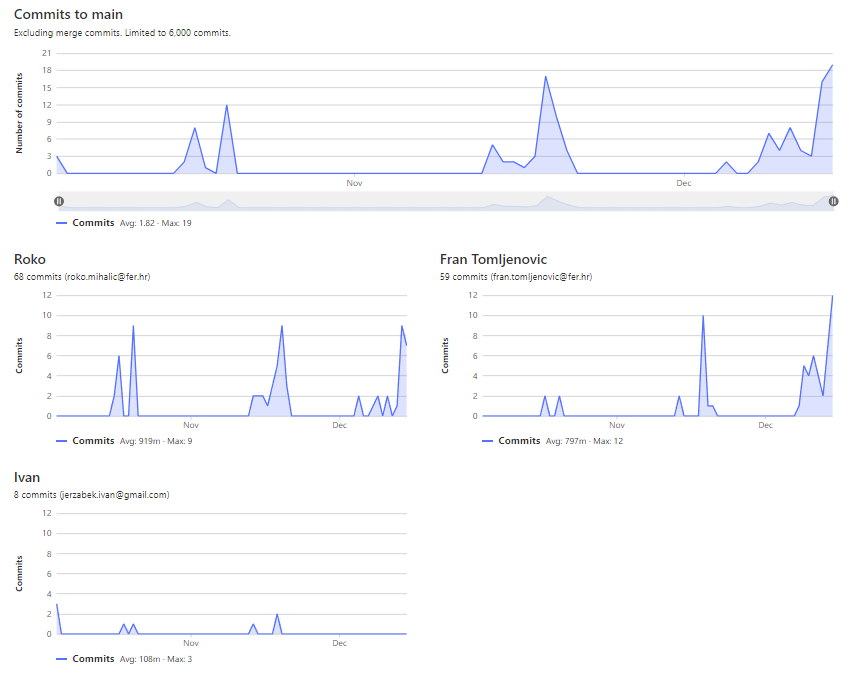
\includegraphics[width=\textwidth]{slike/PrikazAktivnostiNaRepozitorijuPrviDio.png} %veličina u odnosu na širinu linije
			\caption{Prikaz Aktivnosti Na Repozitoriju Prvi Dio}
			\label{fig:PrikazAktivnostiNaRepozitorijuPrviDio} %label mora biti drugaciji za svaku sliku
		\end{figure}
		
		\begin{figure}[H]
			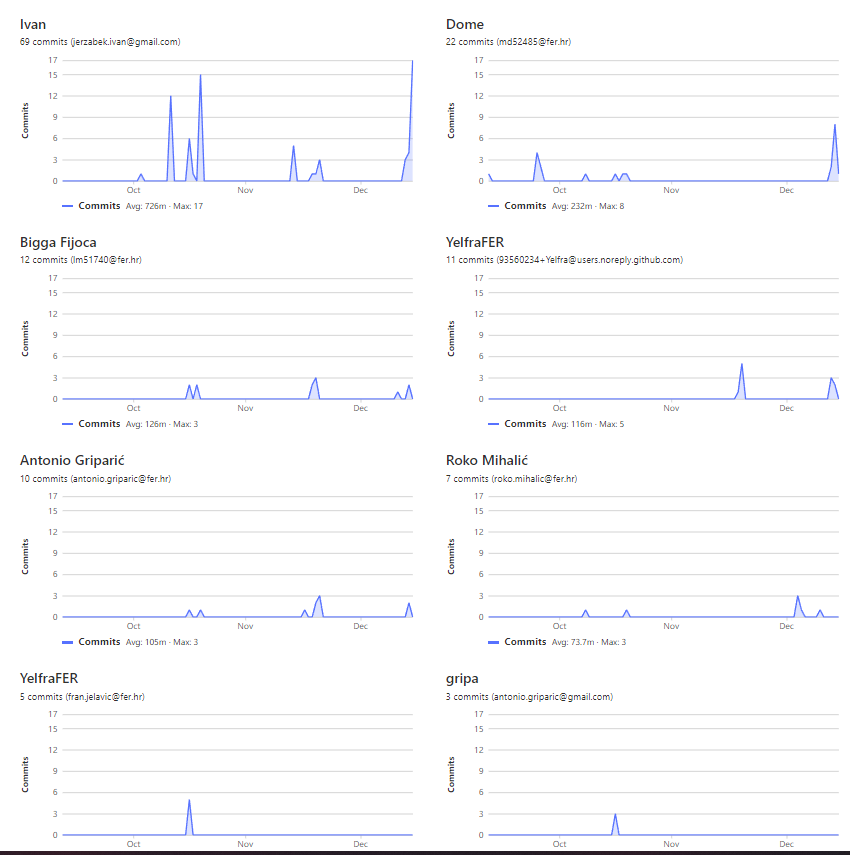
\includegraphics[width=\textwidth]{slike/PrikazAktivnostiNaRepozitorijuDrugiDio.png} %veličina u odnosu na širinu linije
			\caption{Prikaz Aktivnosti Na Repozitoriju Drugi Dio}
			\label{fig:PrikazAktivnostiNaRepozitorijuDrugiDio} %label mora biti drugaciji za svaku sliku
		\end{figure}
	
		
	


\end{document} %naredbe i tekst nakon ove naredbe ne ulaze u izgrađen dokument 


